\documentclass{zjureport}
% \special{dvipdfmx:config z 0} % 取消PDF压缩,加快速度,最终版本生成的时候最好把这句话注释掉
\usepackage{enumitem}
\usepackage{hyperref}
\hypersetup{hypertex=true,colorlinks=true,linkcolor=blue,anchorcolor=blue,citecolor=blue}
% =============================================
% Part 0 Edit the info
% =============================================

\major{信息工程}
\name{东四421-G2}
\partner{何铭源、焦正浩}
\title{本科实验报告}
\stuid{}
\college{信息与电子工程学院}
\date{\today}
\lab{东四421}
\course{电子工程训练(甲)}
\instructor{李培弘}
\grades{}
\expname{智能插座实验}
\exptype{}
\pagestyle{fancy}
\rhead{小组:东四421-G2}
\chead{}

\begin{document}
% =============================================
% Part 1 Header
% =============================================
\makecover

% \makecontent

\makeheader
% =============================================
% Part 2 Main document
% =============================================


\section{新智能插座DIY电装}
\subsection{供电电路测试}
\begin{table}[H]
\centering
\caption{供电测试结果}
\begin{tabular}{L{.7\textwidth}C{.2\textwidth}}
\toprule
检测项目 & 检测结果\\
\midrule
电源空载时的输出电压:  & 5.100V \\
插上电源后D3状态(亮/灭):     & 亮    \\
插上电源后,标注5V处(J1的3脚)的电压: & 5.102V\\
\bottomrule
\end{tabular}
\end{table}
再最开始通上电后,LED灯没有正常亮起,经调试发现LED灯是坏的。借助吸锡器将LED取下后更换新的重试,发现结果正常。
\begin{figure}[H]
\centering
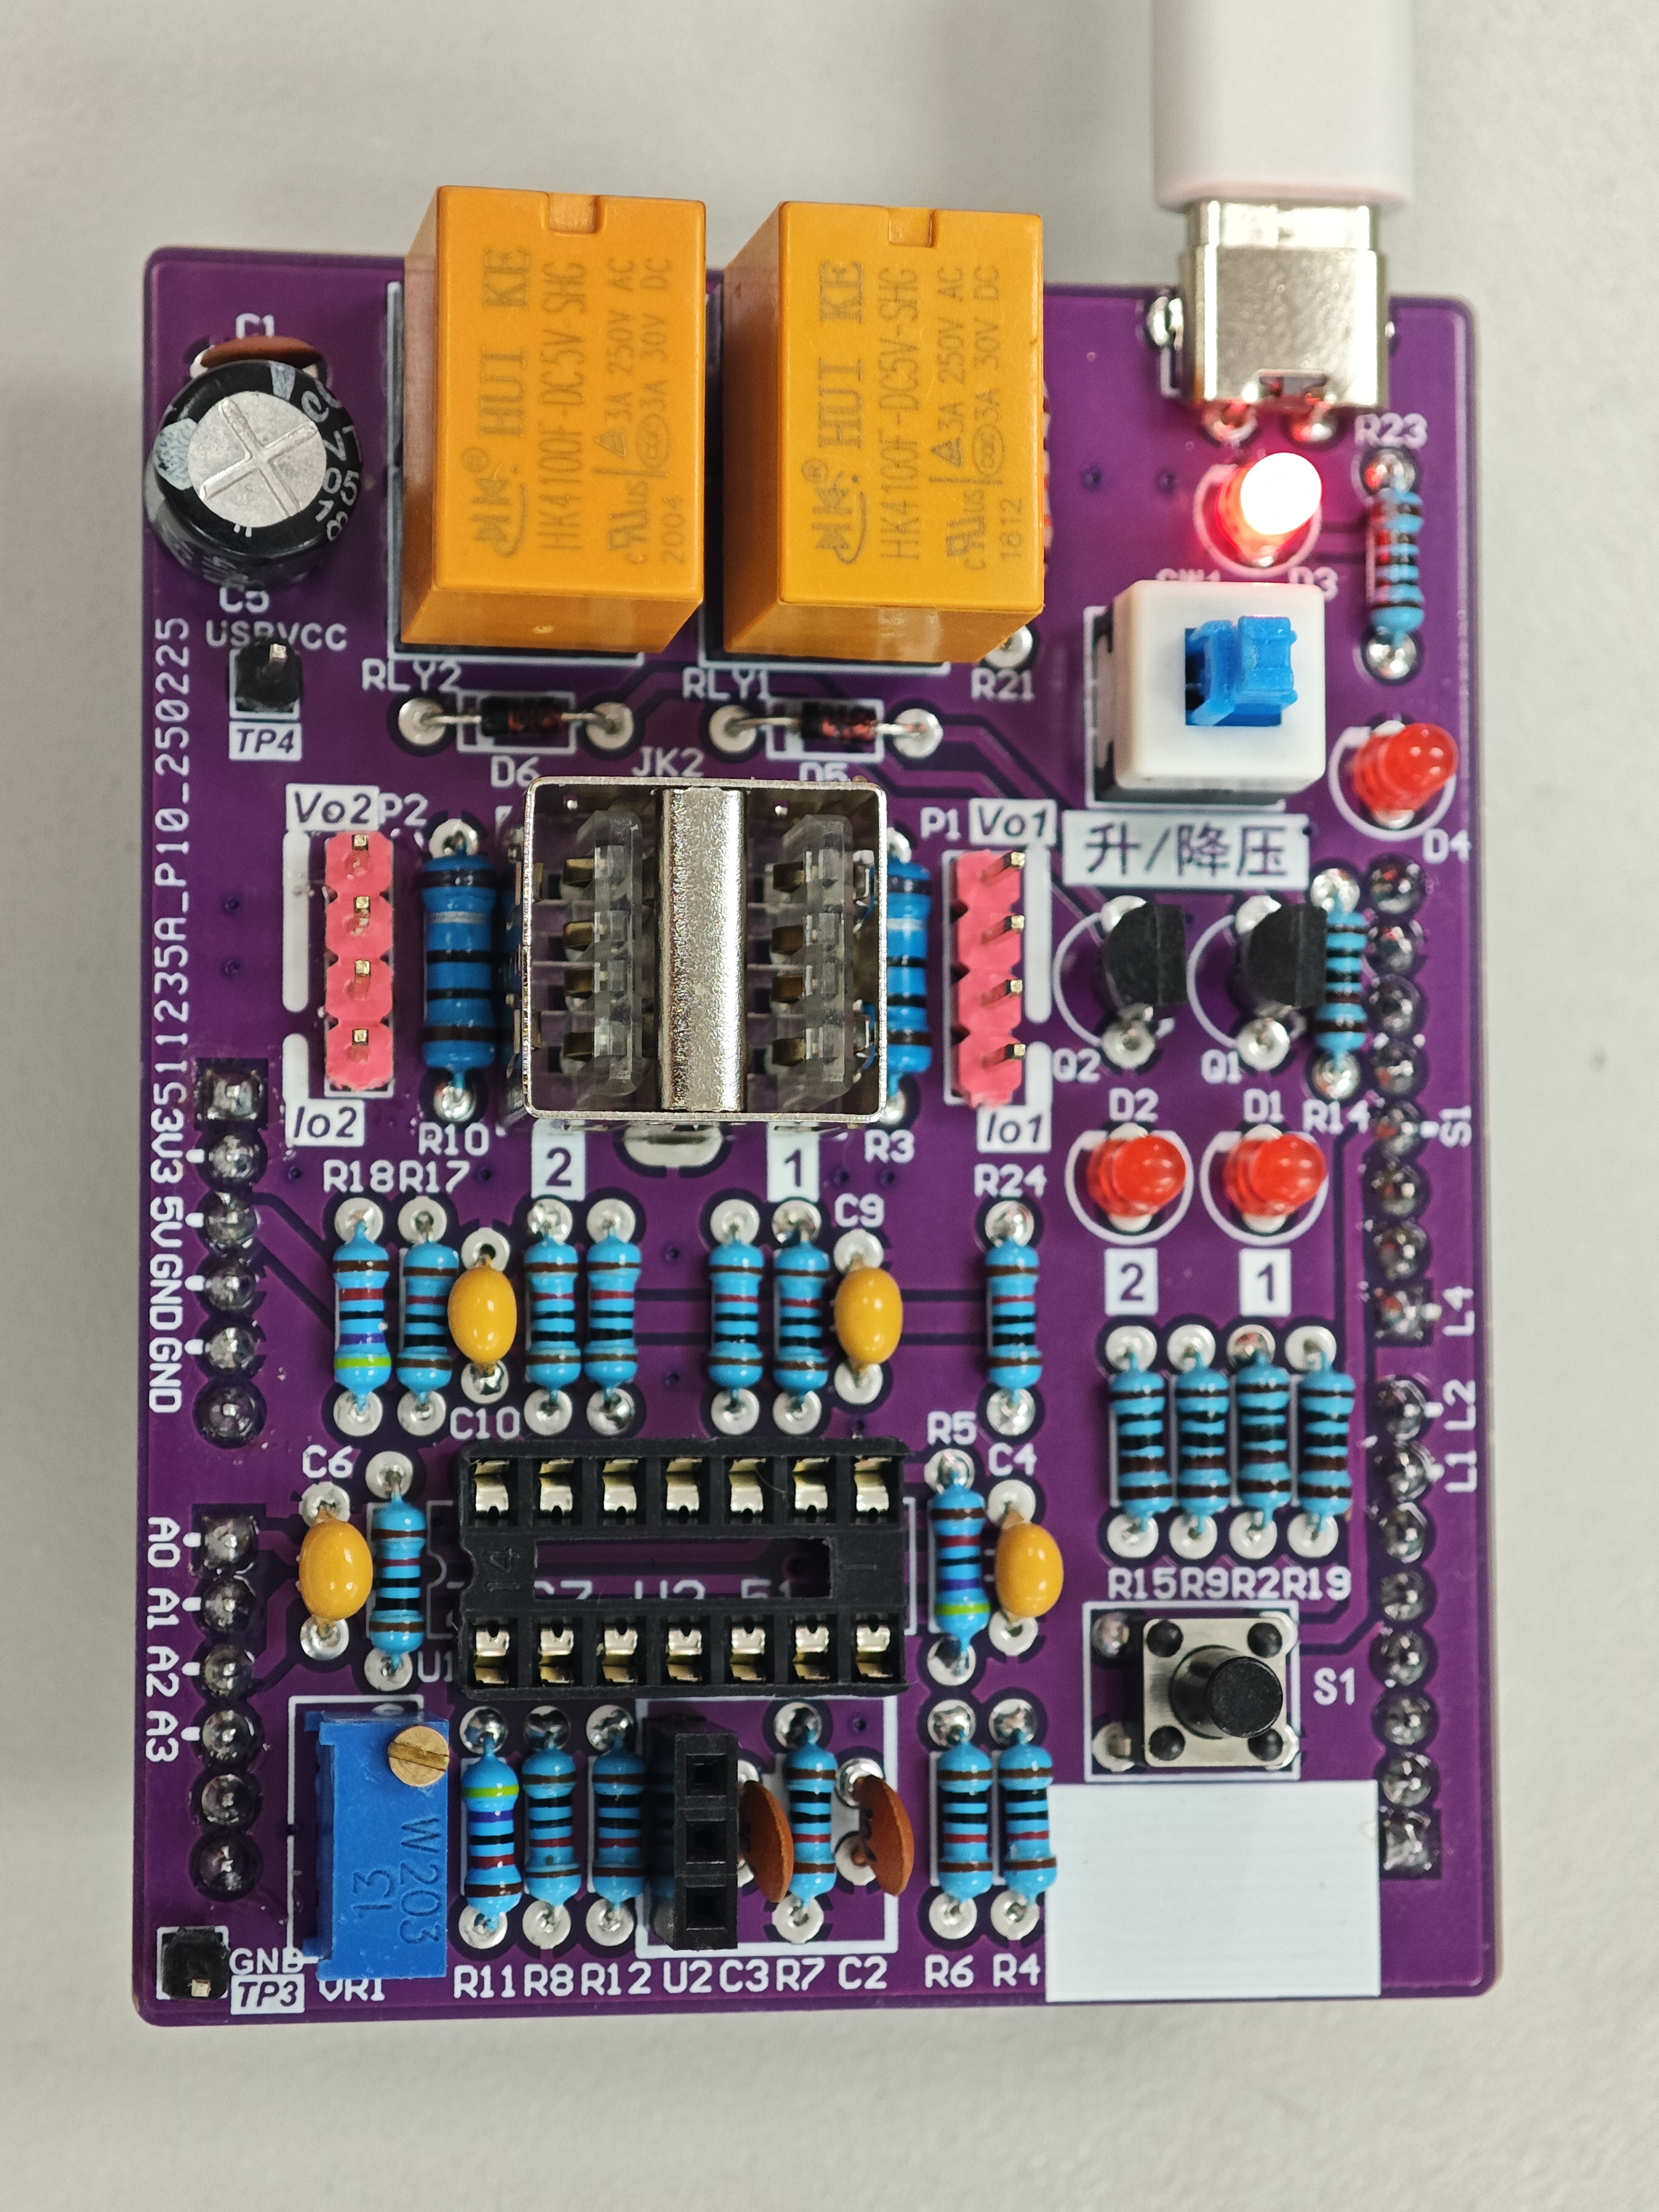
\includegraphics[width=.3\textwidth]{./figures/插座/通电.jpg}
\includegraphics[width=.3\textwidth]{./figures/插座/通电测量.jpg}
\caption{通电测量过程}
\end{figure}
\subsection{USB插座供电控制电路测试}
\textbf{USB供电通路的信号路径}:引脚 IO7 通过高/低电平(即+5V/0V),可控制三极管 Q1 的导通/截止,从而决定继电器 RLY2 的
通断,最终决定 USB 供电插座 JK2 上的 USB2 口是否有 5V(即 USBVCC)电源输出。供电电流将从
USB2 口的 VCC 引脚流出,经过外接用电器,从 USB2 口的 GND 流回。
\begin{table}[H]
\centering
\caption{USB插座供电控制电路测试结果}
\begin{tabular}{L{.4\textwidth}L{.4\textwidth}}
    \toprule
检测项目  & 检测结果 \\
\midrule
以杜邦线连接标注L1处至标注5V,观察到的现象:   & D1\underline{亮},继电器RLY1\underline{吸合},USB供电插座1的供电电压\underline{5.088V}。 \\
以杜邦线连接标注L1处至标注GND,观察到的现象: &    D1\underline{灭},继电器RLY1\underline{断开},USB供电插座1的供电电压\underline{0V}。\\
以杜邦线连接标注L2处至标注5V,观察到的现象:  & D2\underline{亮},继电器RLY2\underline{吸合},USB供电插座2的供电电压\underline{5.087V}。 \\
以杜邦线连接标注L2处至标注GND,观察到的现象:  &  D2\underline{灭},继电器RLY2\underline{断开},USB供电插座2的供电电压\underline{0V}。\\
\bottomrule
\end{tabular}
\end{table}
\begin{figure}[H]
  \centering
  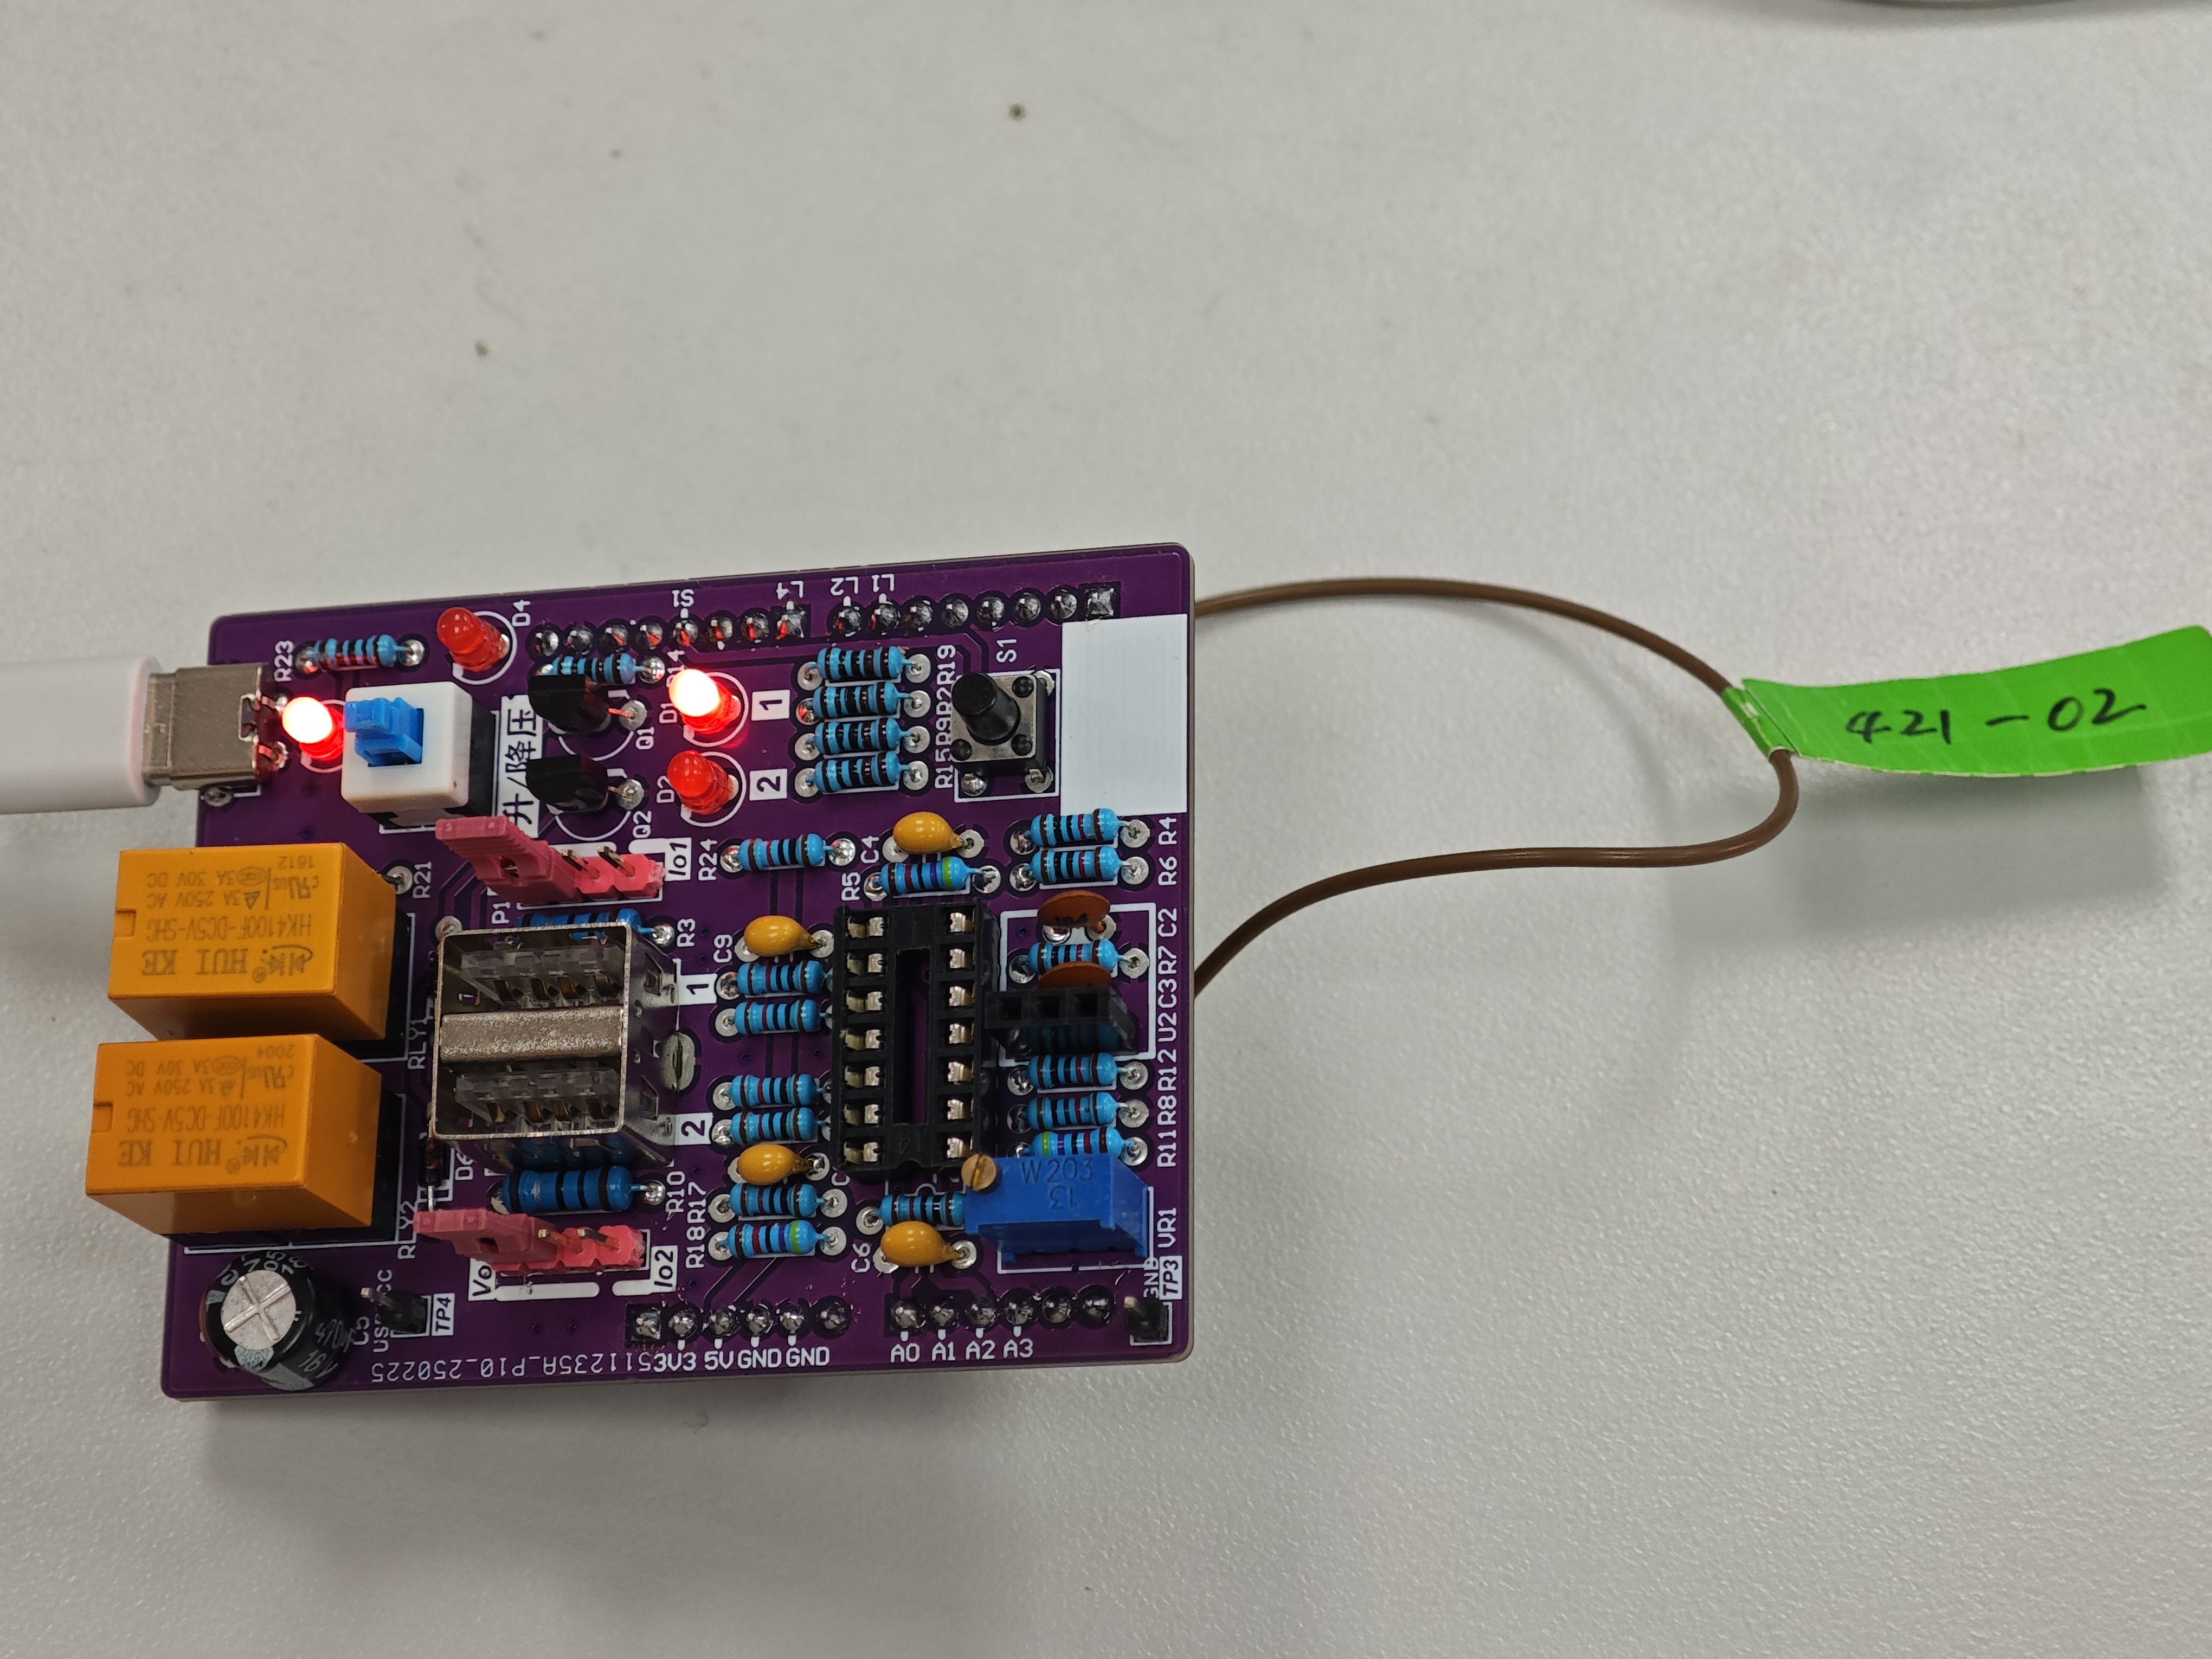
\includegraphics[width=.3\textwidth]{./figures/插座/usb1供电.jpg}
  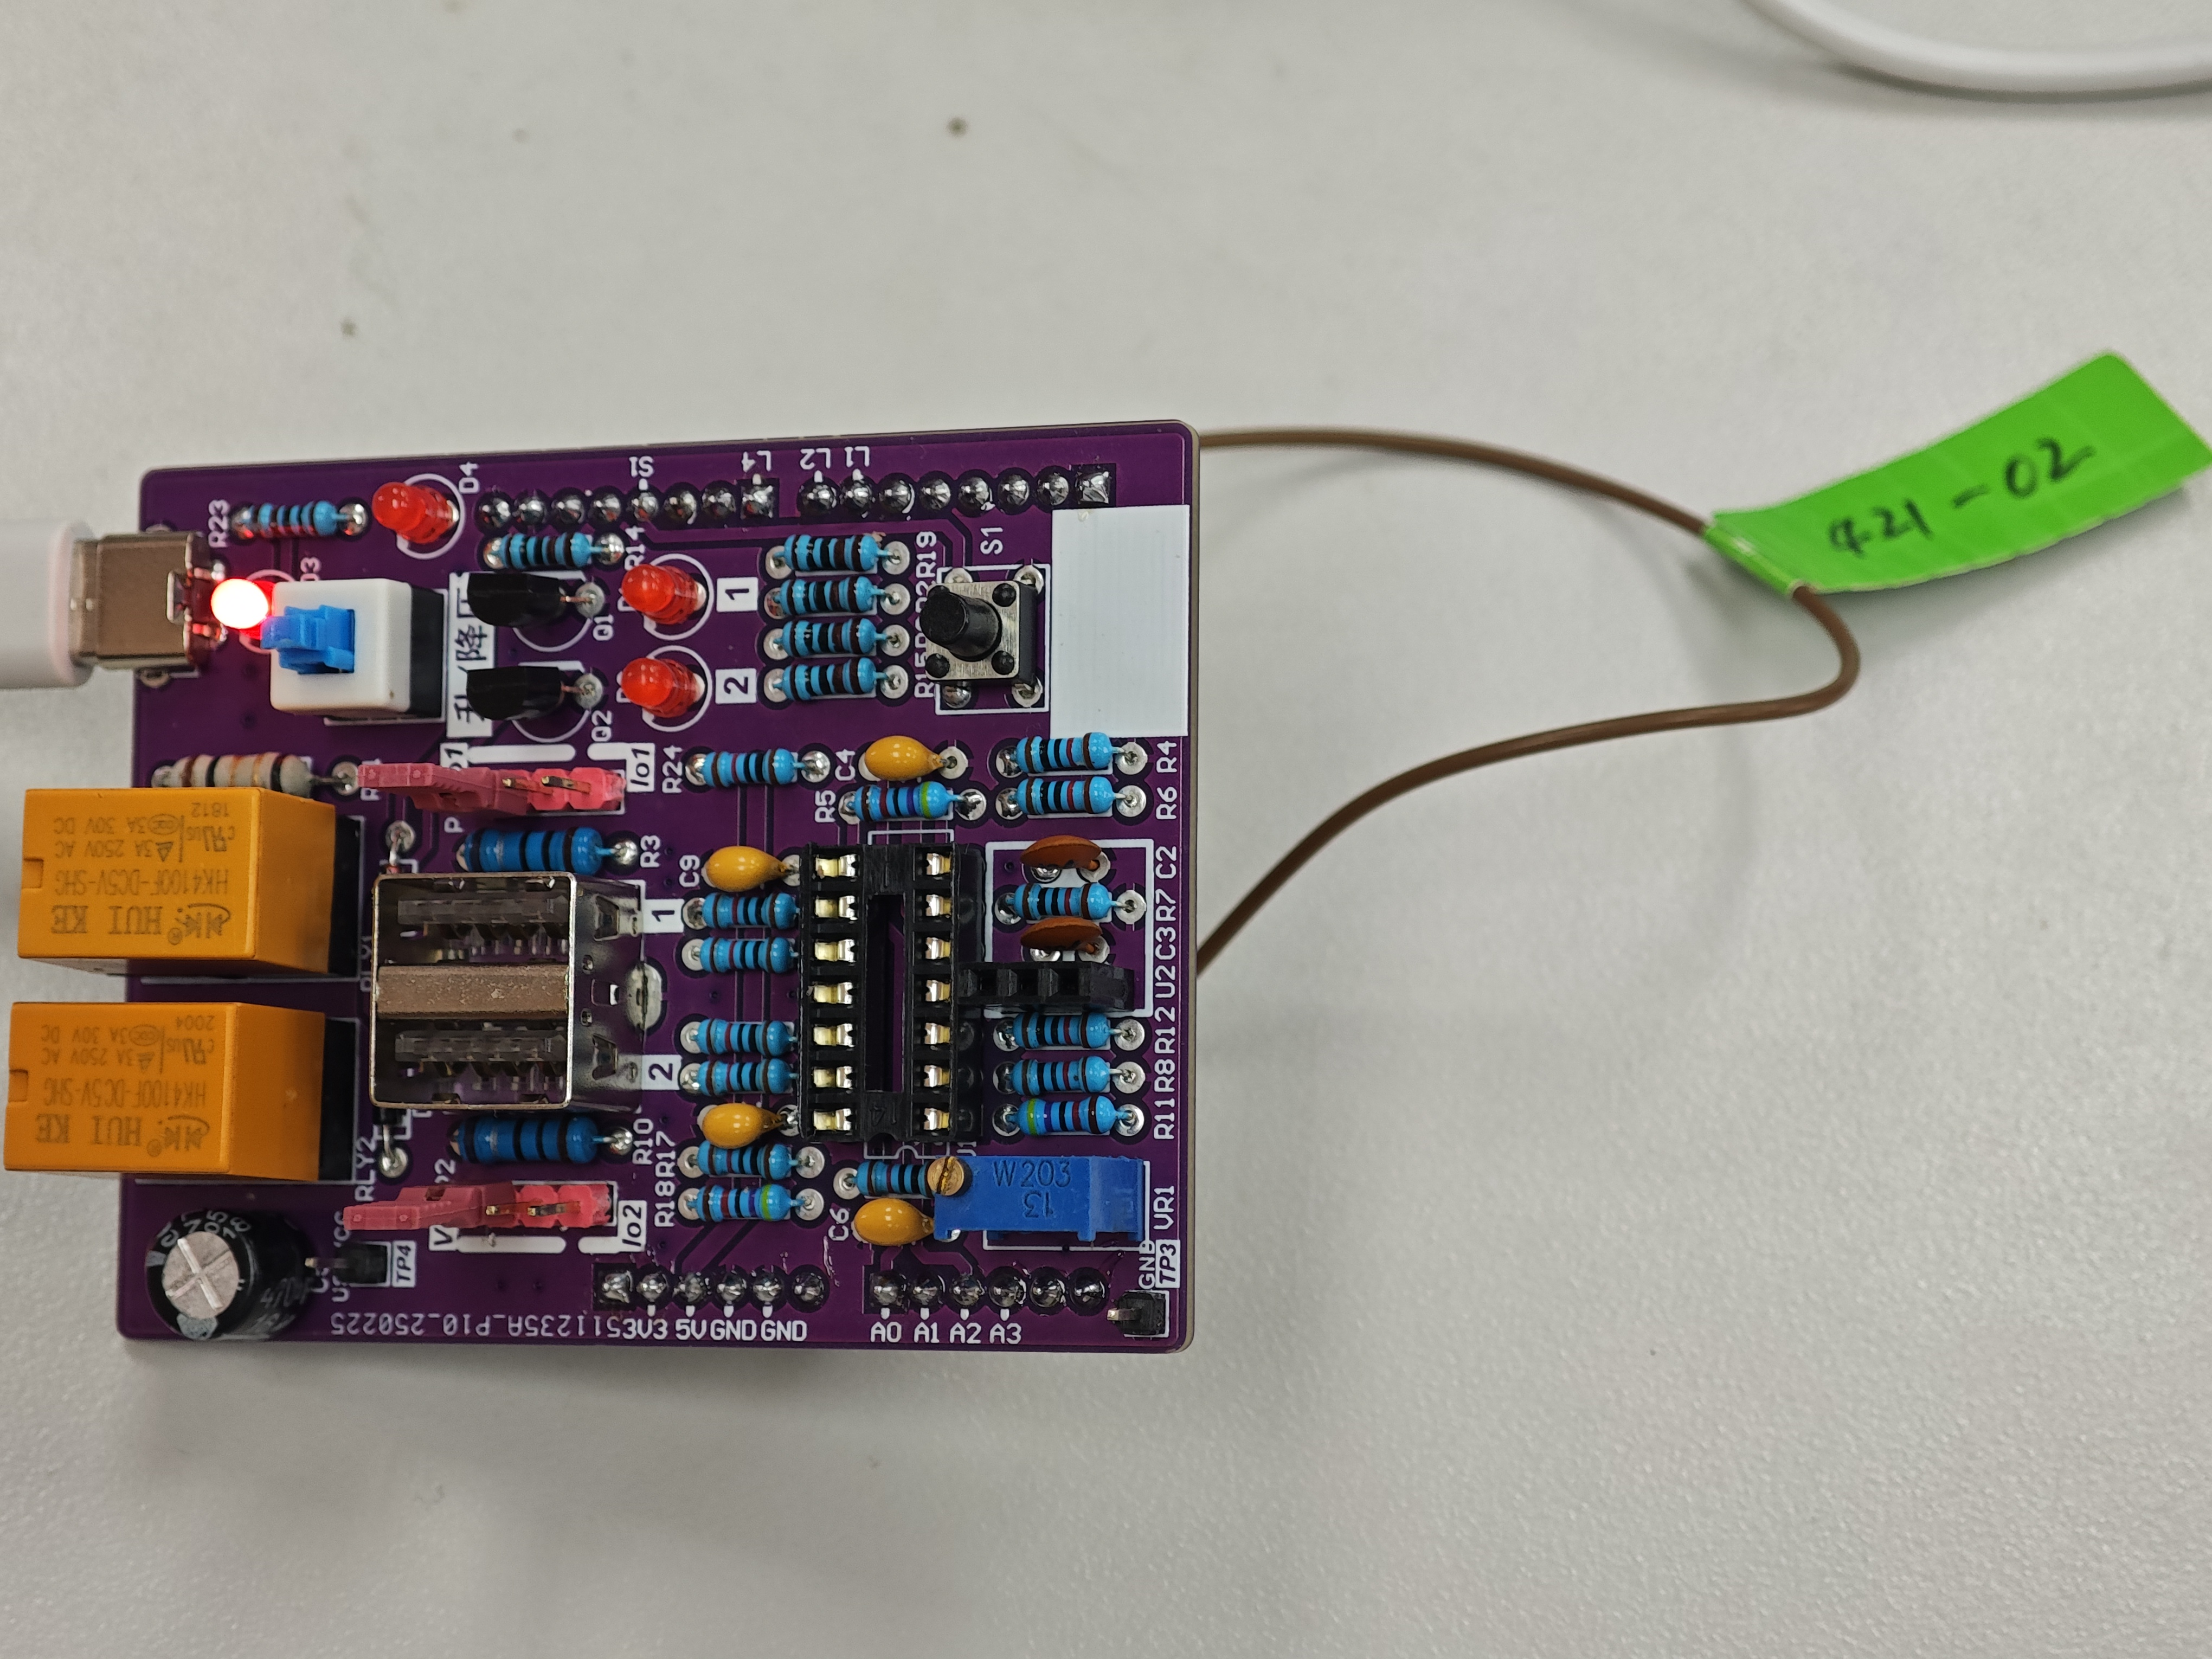
\includegraphics[width=.3\textwidth]{./figures/插座/usb1断电.jpg}
  \caption{L1,继电器RLY1测试}
\end{figure}
\begin{figure}[H]
  \centering
  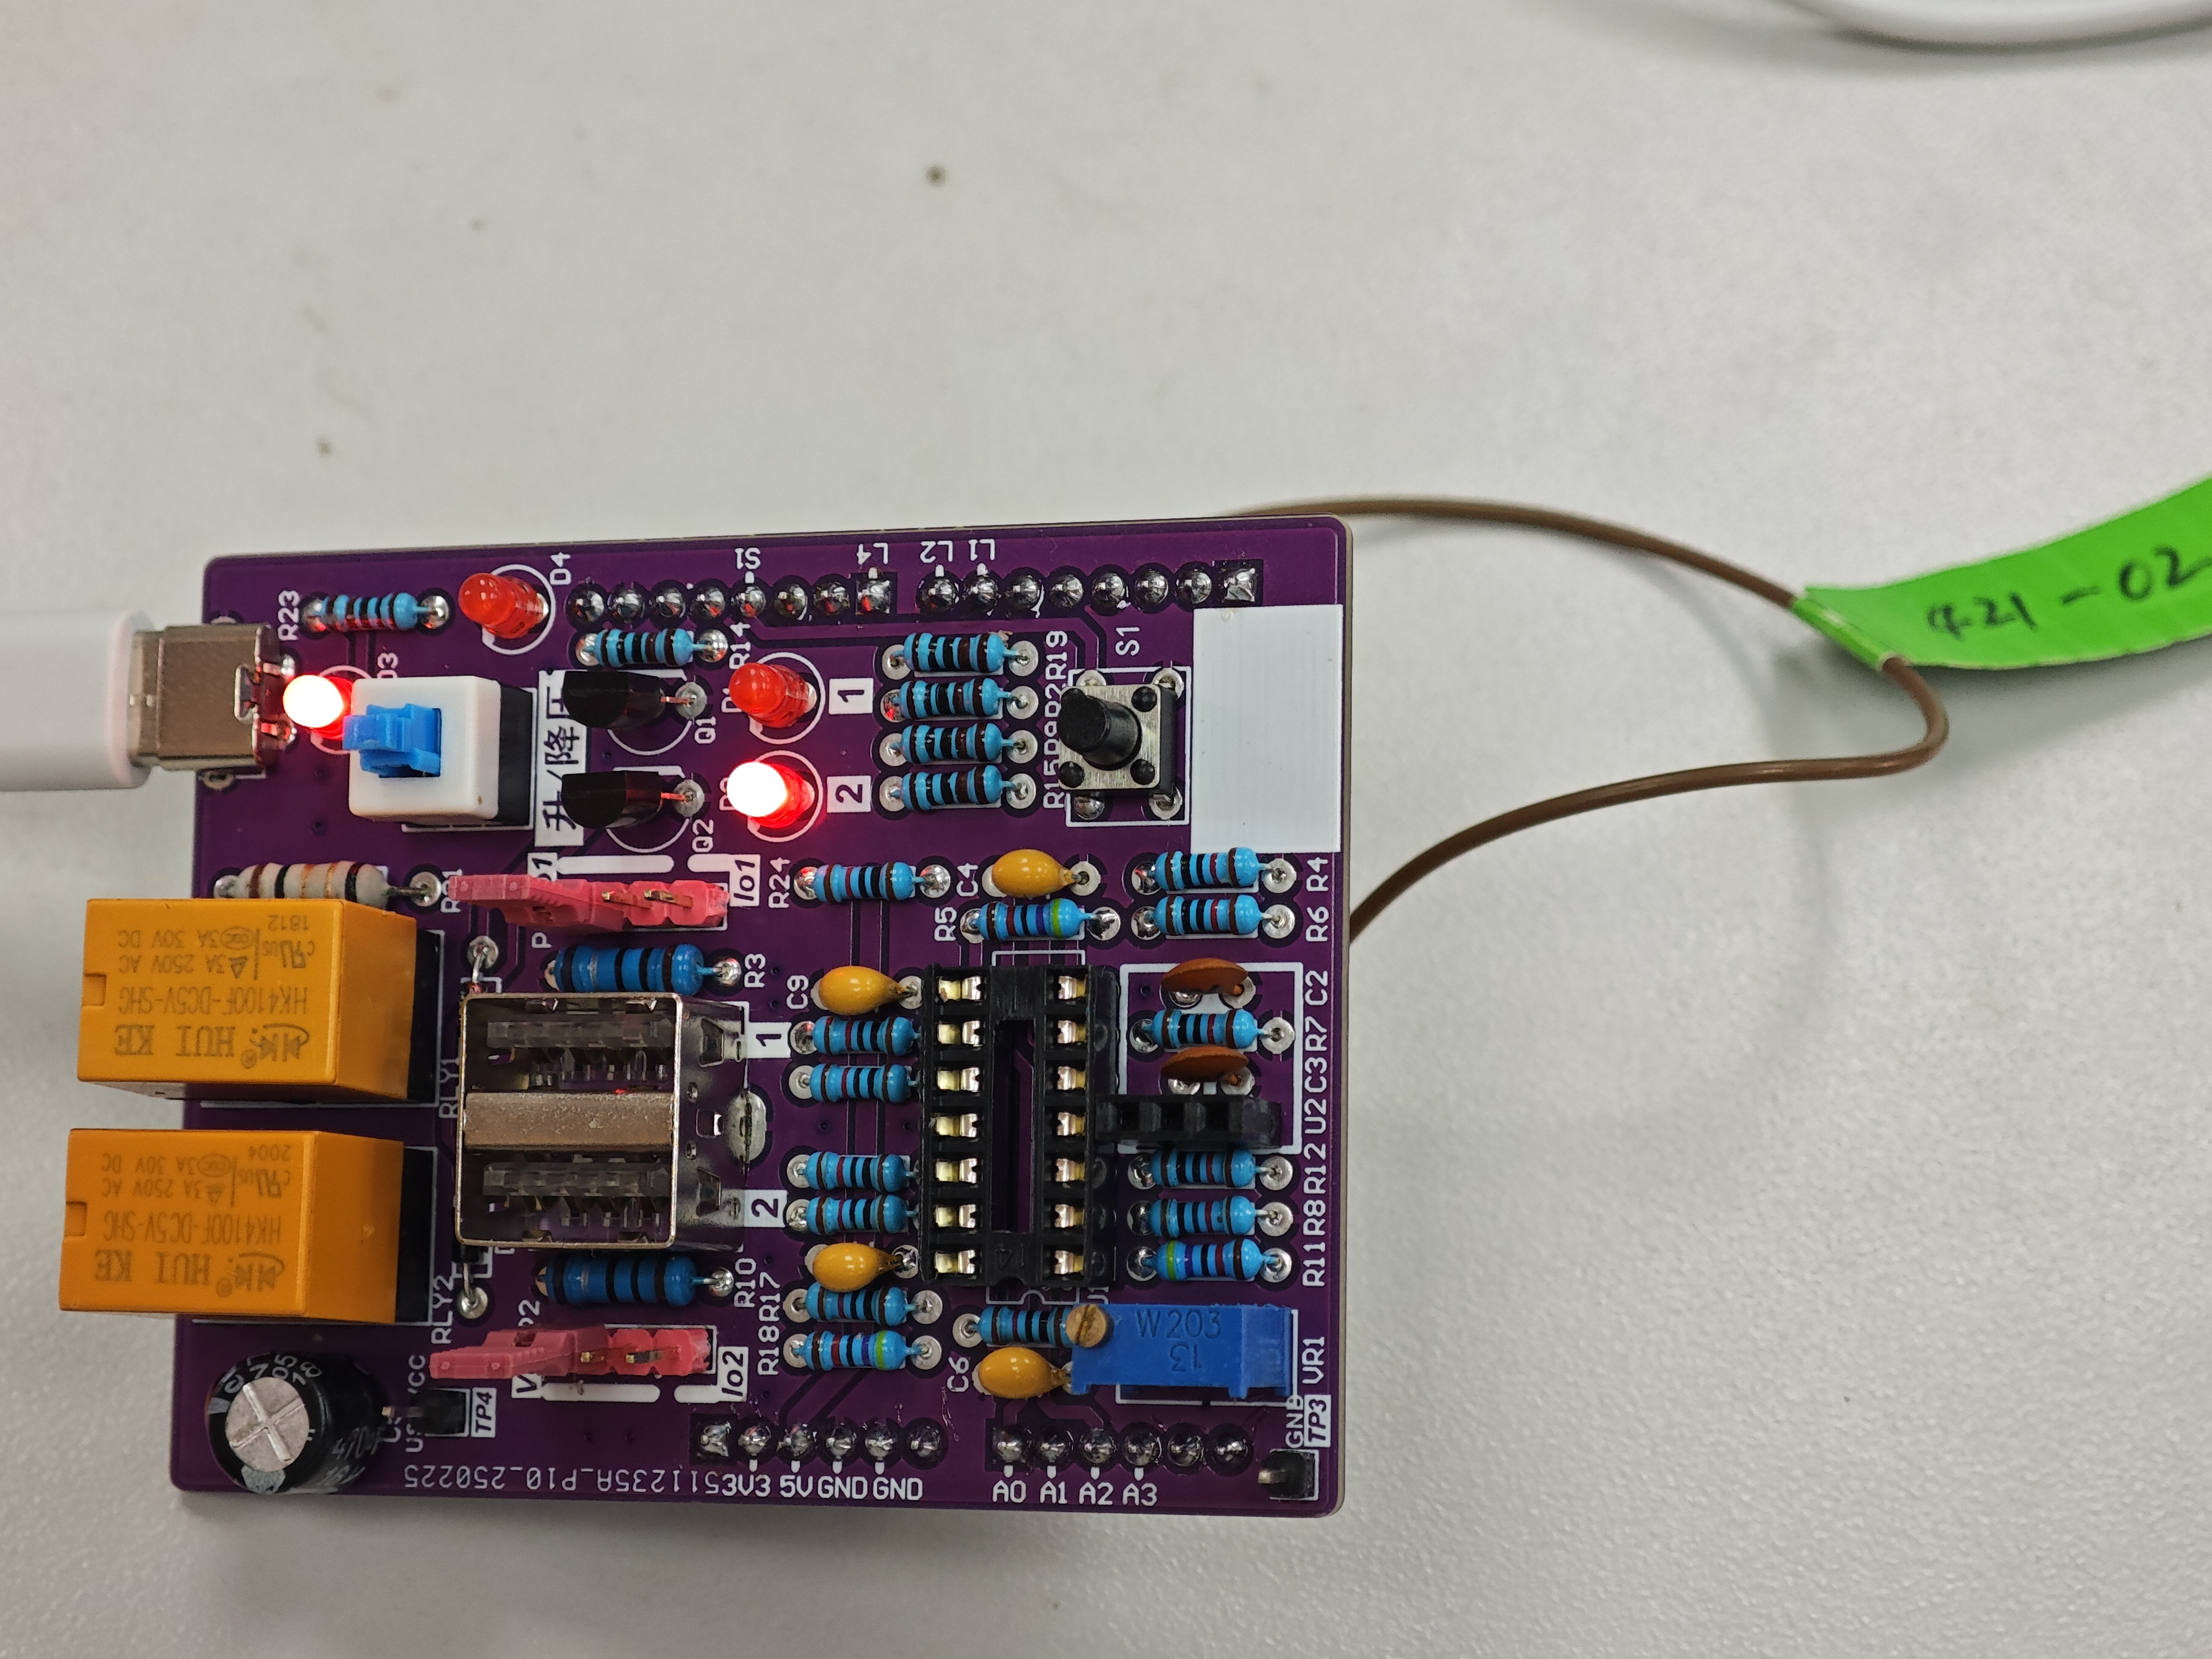
\includegraphics[width=.3\textwidth]{./figures/插座/usb2通电.jpg}
  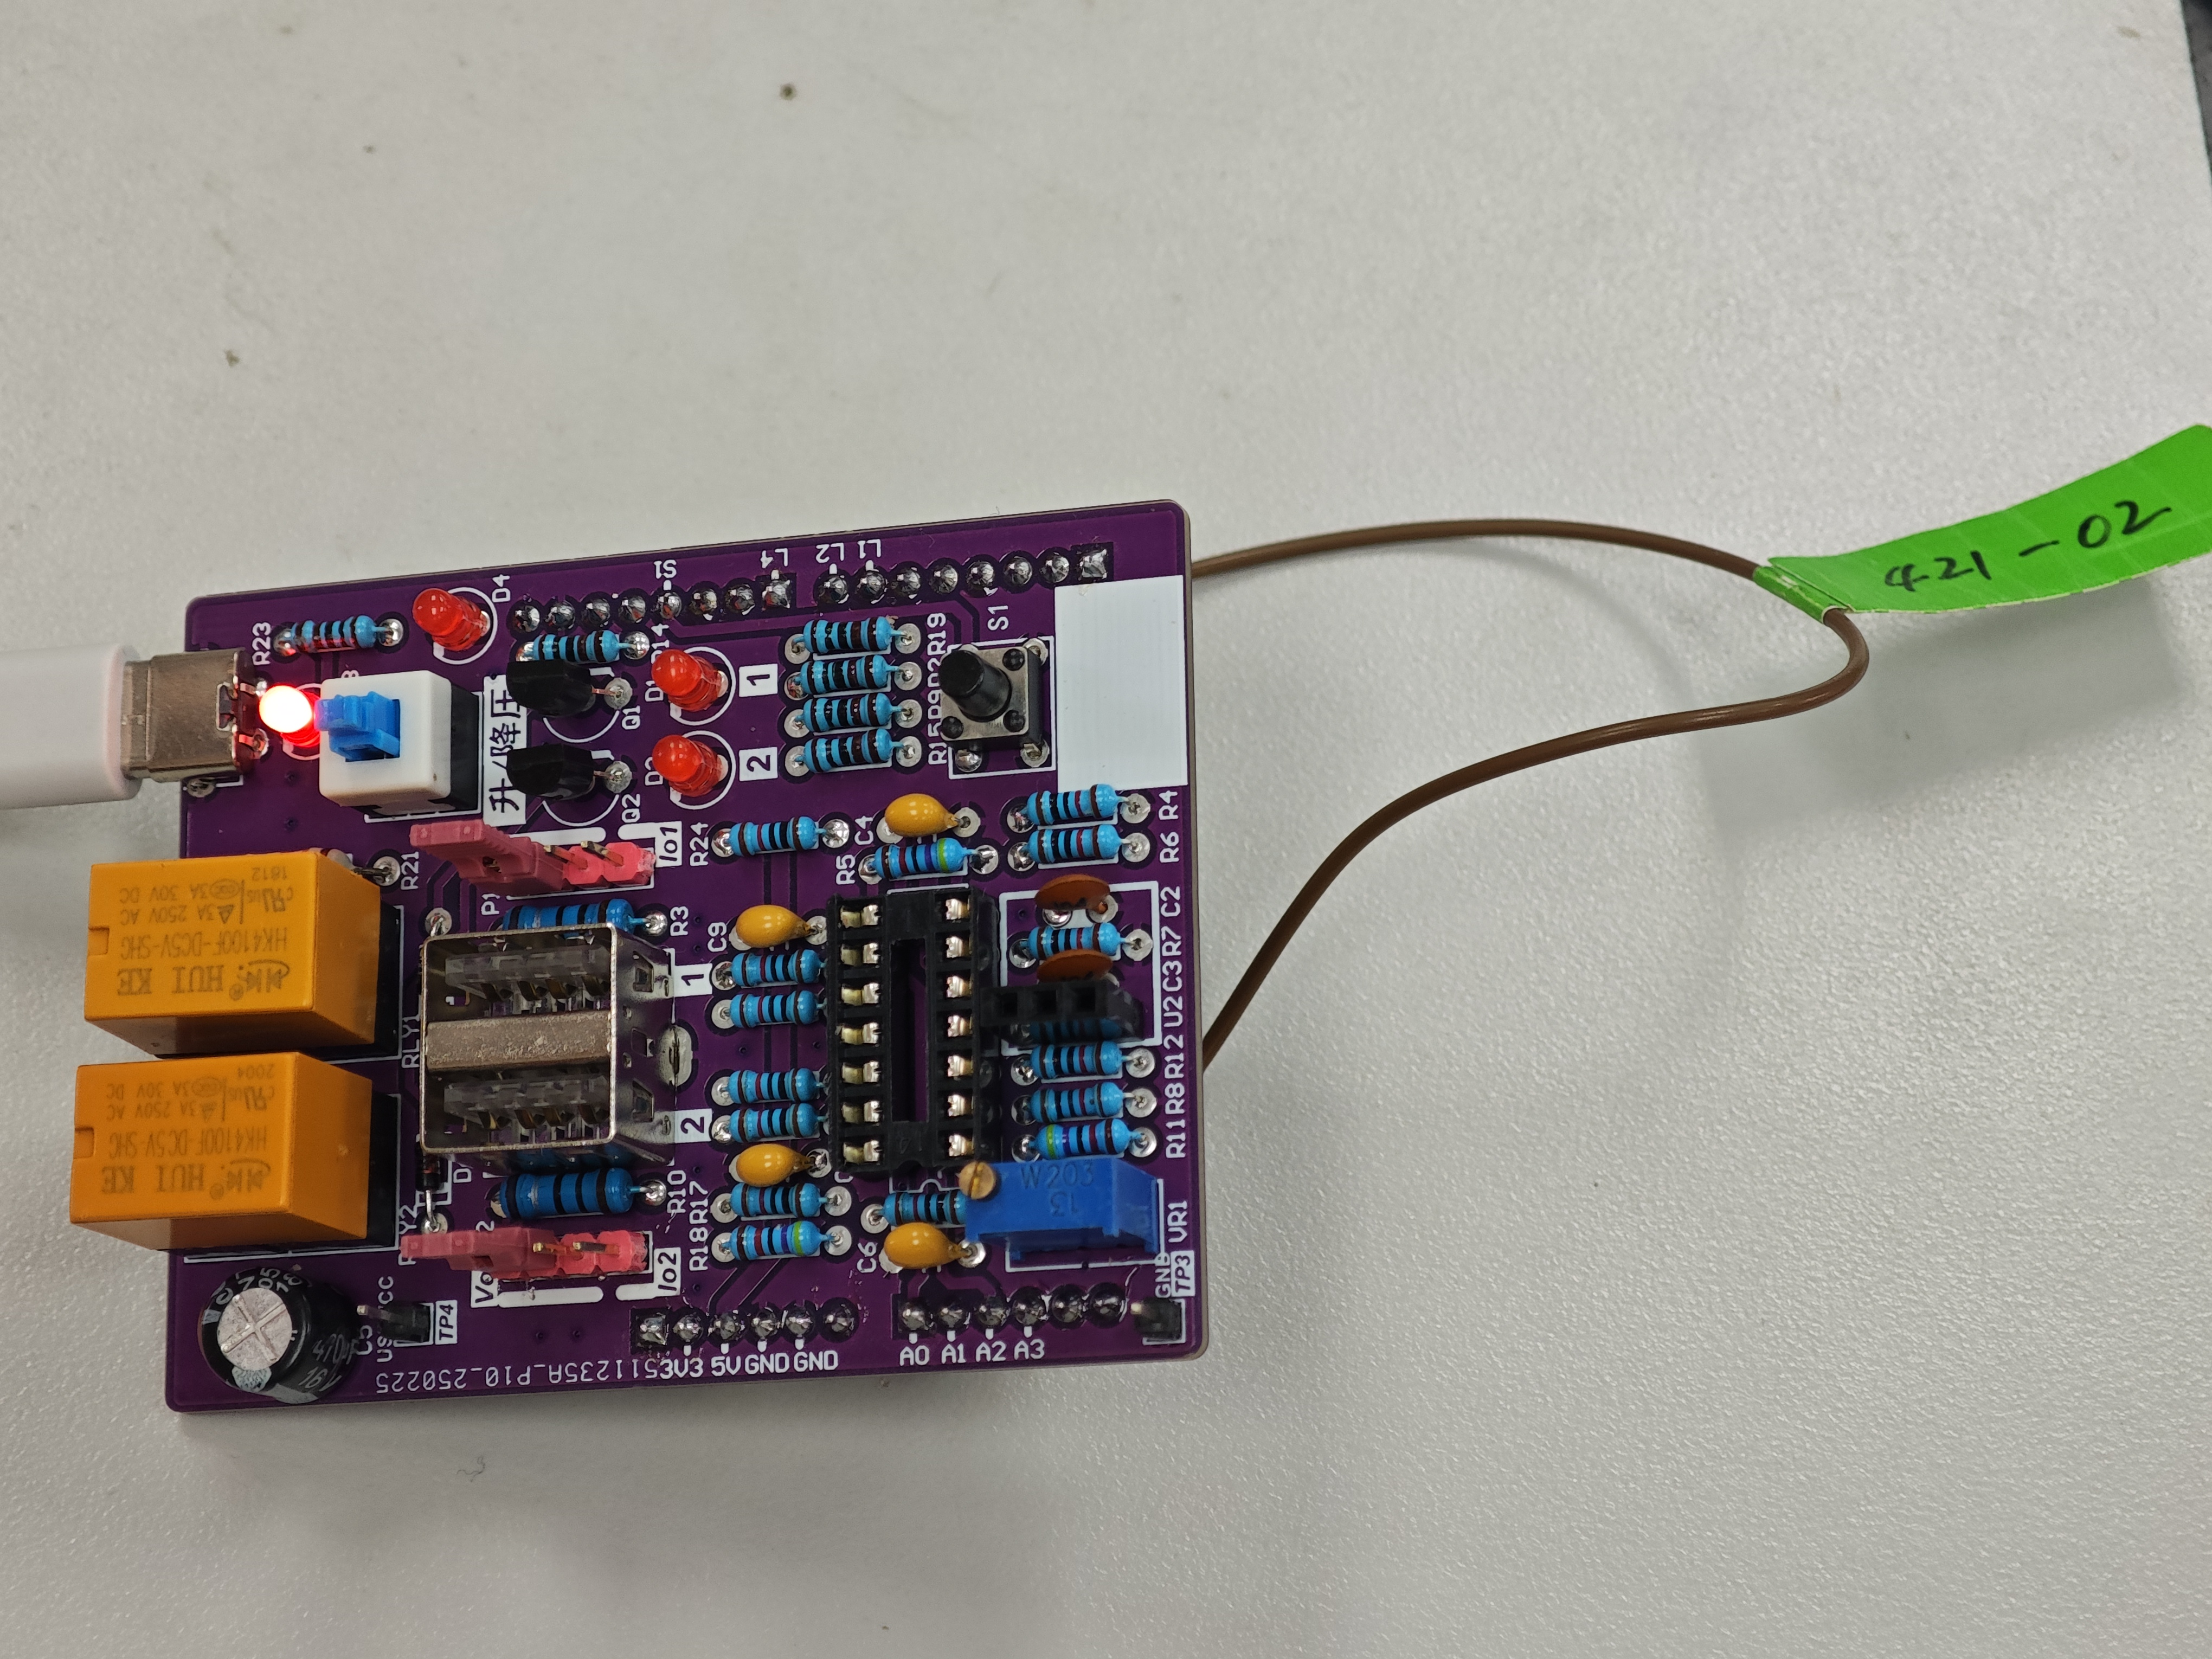
\includegraphics[width=.3\textwidth]{./figures/插座/usb2断电.jpg}
  \caption{L2,继电器RLY2测试}
\end{figure}
\subsection{指示灯测试}
\begin{table}[H]
\centering
\caption{指示灯测试结果}
\begin{tabular}{L{.4\textwidth}L{.4\textwidth}}
\toprule
检测项目  & 检测结果 \\
\midrule
电路上电,以杜邦线连接标注L4处至标注5V,观察到的现象:  & D4\underline{亮}。这里通过标注4所施加的5V电压,就是后续系统能通过软件输出的二进制控制信号``1''。 \\
电路上电,以杜邦线连接标注L4处至标注GND,观察到的现象:  & D4\underline{灭}。这里通过标注4所施加的0V电压,就是后续系统能通过软件输出的二进制控制信号``0''。 \\
\bottomrule
\end{tabular}
\end{table}
\begin{figure}[H]
\centering
 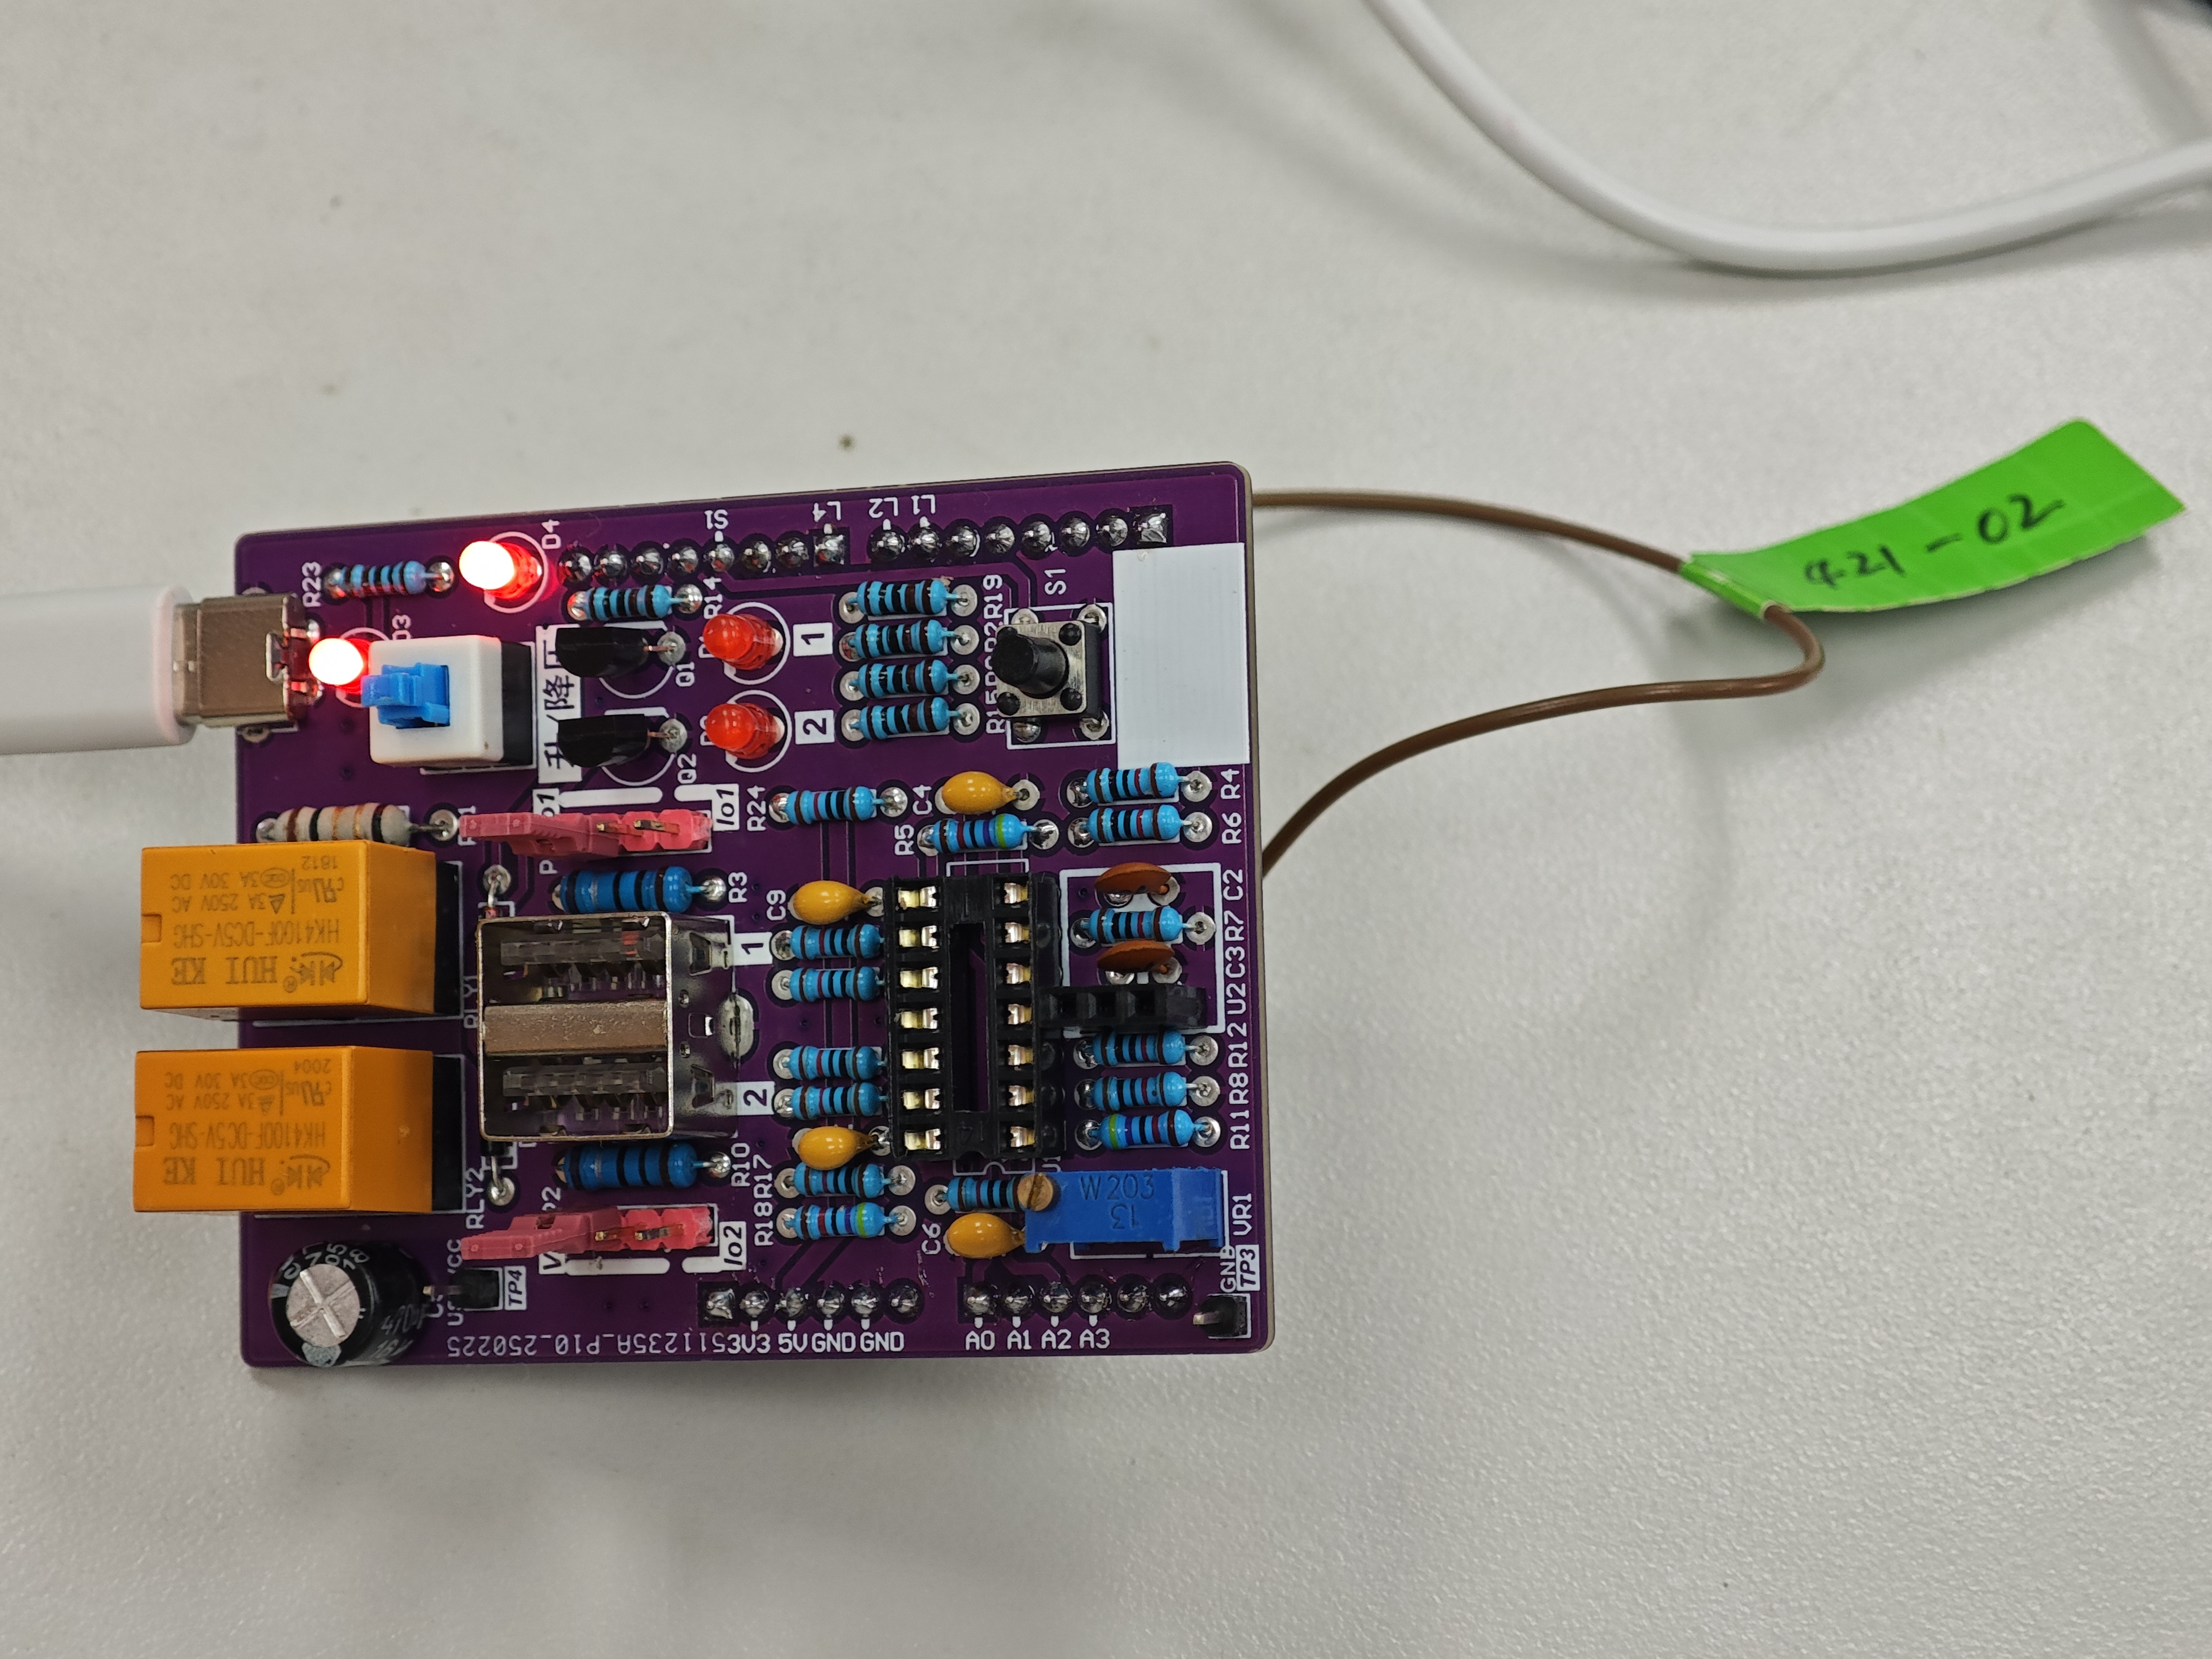
\includegraphics[width=.5\textwidth]{./figures/插座/控制D4.jpg}
 \caption{控制L4亮起}
\end{figure}
\subsection{集成电路芯片的供电检测}
\begin{table}[H]
    \centering
    \caption{集成电路芯片的供电检测结果}
    \begin{tabular}{L{.6\textwidth}C{.2\textwidth}}
    \toprule
    检测项目  & 检测结果 \\
    \midrule
    LM324AN 的电源电压(V): & 5.092V \\
    LM35DZ 的电源电压(V): &  5.103V \\
    \bottomrule
    \end{tabular}
    \end{table}
    \begin{figure}[H]
        \centering
         \includegraphics[width=.3\textwidth]{./figures/插座/集成电路供电.jpg}
         \hspace{5em}
         \includegraphics[width=.3\textwidth]{./figures/插座/温度传感器供电.jpg}
         \caption{测量集成电路供电}
        \end{figure}
\section{新智能插座DIY调试}
\subsection{基于硬件调整的温度值标定调试}
通过调整可变电阻VR1的值,改变温度传感器读取的数值。从$28.6\textcelsius$调整为$31.0\textcelsius$。
\begin{table}[H]
  \centering
  \caption{温度值标定调试结果}
  \begin{tabular}{L{0.4\textwidth}C{.4\textwidth}}
    \toprule
    项目  & 测量值\\
    \midrule
    当前实际室温  & 31.1\textcelsius \\
    经你完成调试后测试程序显示温度  & 31.0\textcelsius \\
    是否存在严重的元器件离散性问题?  & 否\\
    \bottomrule
  \end{tabular}
\end{table}
\subsection{基于软件后处理的电流数据标定}
利用多组数据,通过线性回归计算出软件读取值与实际值的线性关系,从而在软件层面实现数据矫正。
通过串接电子负载,可以调整USB接口输出的电流值,从而得到多组数据。
\begin{table}[H]
\centering
\caption{采样得到的电流数据}
\begin{tabular}{C{.4\textwidth}C{.4\textwidth}}
  \toprule
  Val(串口读取值) & I(实际值)\\
  \midrule
  457mA & 78.3mA\\
  609mA & 105.0mA\\
  \bottomrule
\end{tabular}
\end{table}
可见串口读取值与实际值有较大偏差,通过计算直线方程得
\begin{equation*}
y = 0.1737x - 1.021
\end{equation*}
\begin{lstlisting}[language=C++,caption={修改过后的代码},captionpos=b]
  Serial.print("Socket #1 current: ");
  Serial.print((float)Sensor0*0.173793-1.02102156);
  Serial.print(" mA");
  Serial.print("\t\t");
  Serial.print("Socket #2 current: ");
  Serial.print((float)Sensor1*0.1754680838-2.017431873);
  Serial.println(" mA");
\end{lstlisting}
利用标定好的程序进行测量
\begin{table}[H]
  \centering
  \caption{重新测量并计算误差}
  \begin{tabular}{C{.3\textwidth}C{.3\textwidth}C{.2\textwidth}}
    \toprule
    Val(串口读取值) & I(实际值) & 误差\\
    \midrule
    109.34 & 108.9 & 0.40\%  \\
    93.87  & 93.5  & 0.40\%  \\
    122.89 & 122.9 & 0.01\% \\
    139.49 & 139.5 & 0.01\% \\
    156.09 & 155.7 & 0.25\%  \\
    181.29 & 181.6 & 0.17\% \\
    232.04 & 230.9 & 0.49\%  \\
    384.28 & 382.4 & 0.49\% \\
    \bottomrule
  \end{tabular}
  \end{table}
可见误差已经很小了,仿照1的过程,我们也完成了另一条电路的标定。
\section{软硬件相结合的系统调试}
\subsection{测试任务一}
\begin{table}[H]
\centering
\caption{测试任务1}
\begin{tabular}{L{.2\textwidth}L{.3\textwidth}L{.3\textwidth}}
  \toprule
  输出命令  & 1\#和2\#插座的状态  & 控制电压\\
  \midrule
  发送字符A & 智能插座1\#插座的输出电压,P1的电压:\underline{5.138}V  & J3的\underline{L1}脚电压:\underline{2.925}V\\
  发送字符a & 智能插座1\#插座的输出电压,P1的电压:\underline{0}V  & J3的\underline{L1}脚电压:\underline{0}V\\
  发送字符B & 智能插座2\#插座的输出电压,P2的电压:\underline{5.127}V  & J3的\underline{L2}脚电压:\underline{2.929}V\\
  发送字符b & 智能插座2\#插座的输出电压,P2的电压:\underline{0}V  & J3的\underline{L2}脚电压:\underline{0}V\\
  \bottomrule
\end{tabular}
\end{table}
\subsection{测试任务二}
\begin{table}[H]
  \centering
  \caption{测试任务2}
  \begin{tabular}{L{.3\textwidth}C{.3\textwidth}L{.1\textwidth}}
    \toprule
    项目  & 测量值  & 单位\\
    \midrule
    1\#插座外接的用电器 & \multicolumn{2}{c}{小台灯} \\
    1\#插座电流值 & 196.23  & mA\\
    2\#插座外接的用电器 & \multicolumn{2}{c}{可调光台灯}\\
    2\#插座电流值(最亮时) & 210.83  & mA\\
    2\#插座电流值(最暗时) & 40.52 & mA\\
    插座电压值  & 4.918 & V\\
    温度测量值(环境温度)  & 28.62 & \textcelsius\\
    温度测量值(手指触摸温度)  & 30.3  & \textcelsius\\
    \bottomrule
  \end{tabular}
  \end{table}
\subsection{测试任务三}
将2\#插座上的可调光台灯换成风扇,并接通风扇的插座电源,测量风扇的各档工作电流值。
\begin{table}[H]
\centering
\caption{测试任务3}
\begin{tabular}{L{.3\textwidth}C{.3\textwidth}L{.1\textwidth}}
  \toprule
  项目  & 测量值  & 单位\\
  \midrule
  风扇慢速档电流值 &  239.51  & mA\\
  风扇中速档电流值 &  361.16  & mA\\
  风扇快速档电流值 &  422.51  & mA\\
  \bottomrule
\end{tabular}
\end{table}
\begin{figure}[H]
  \centering
  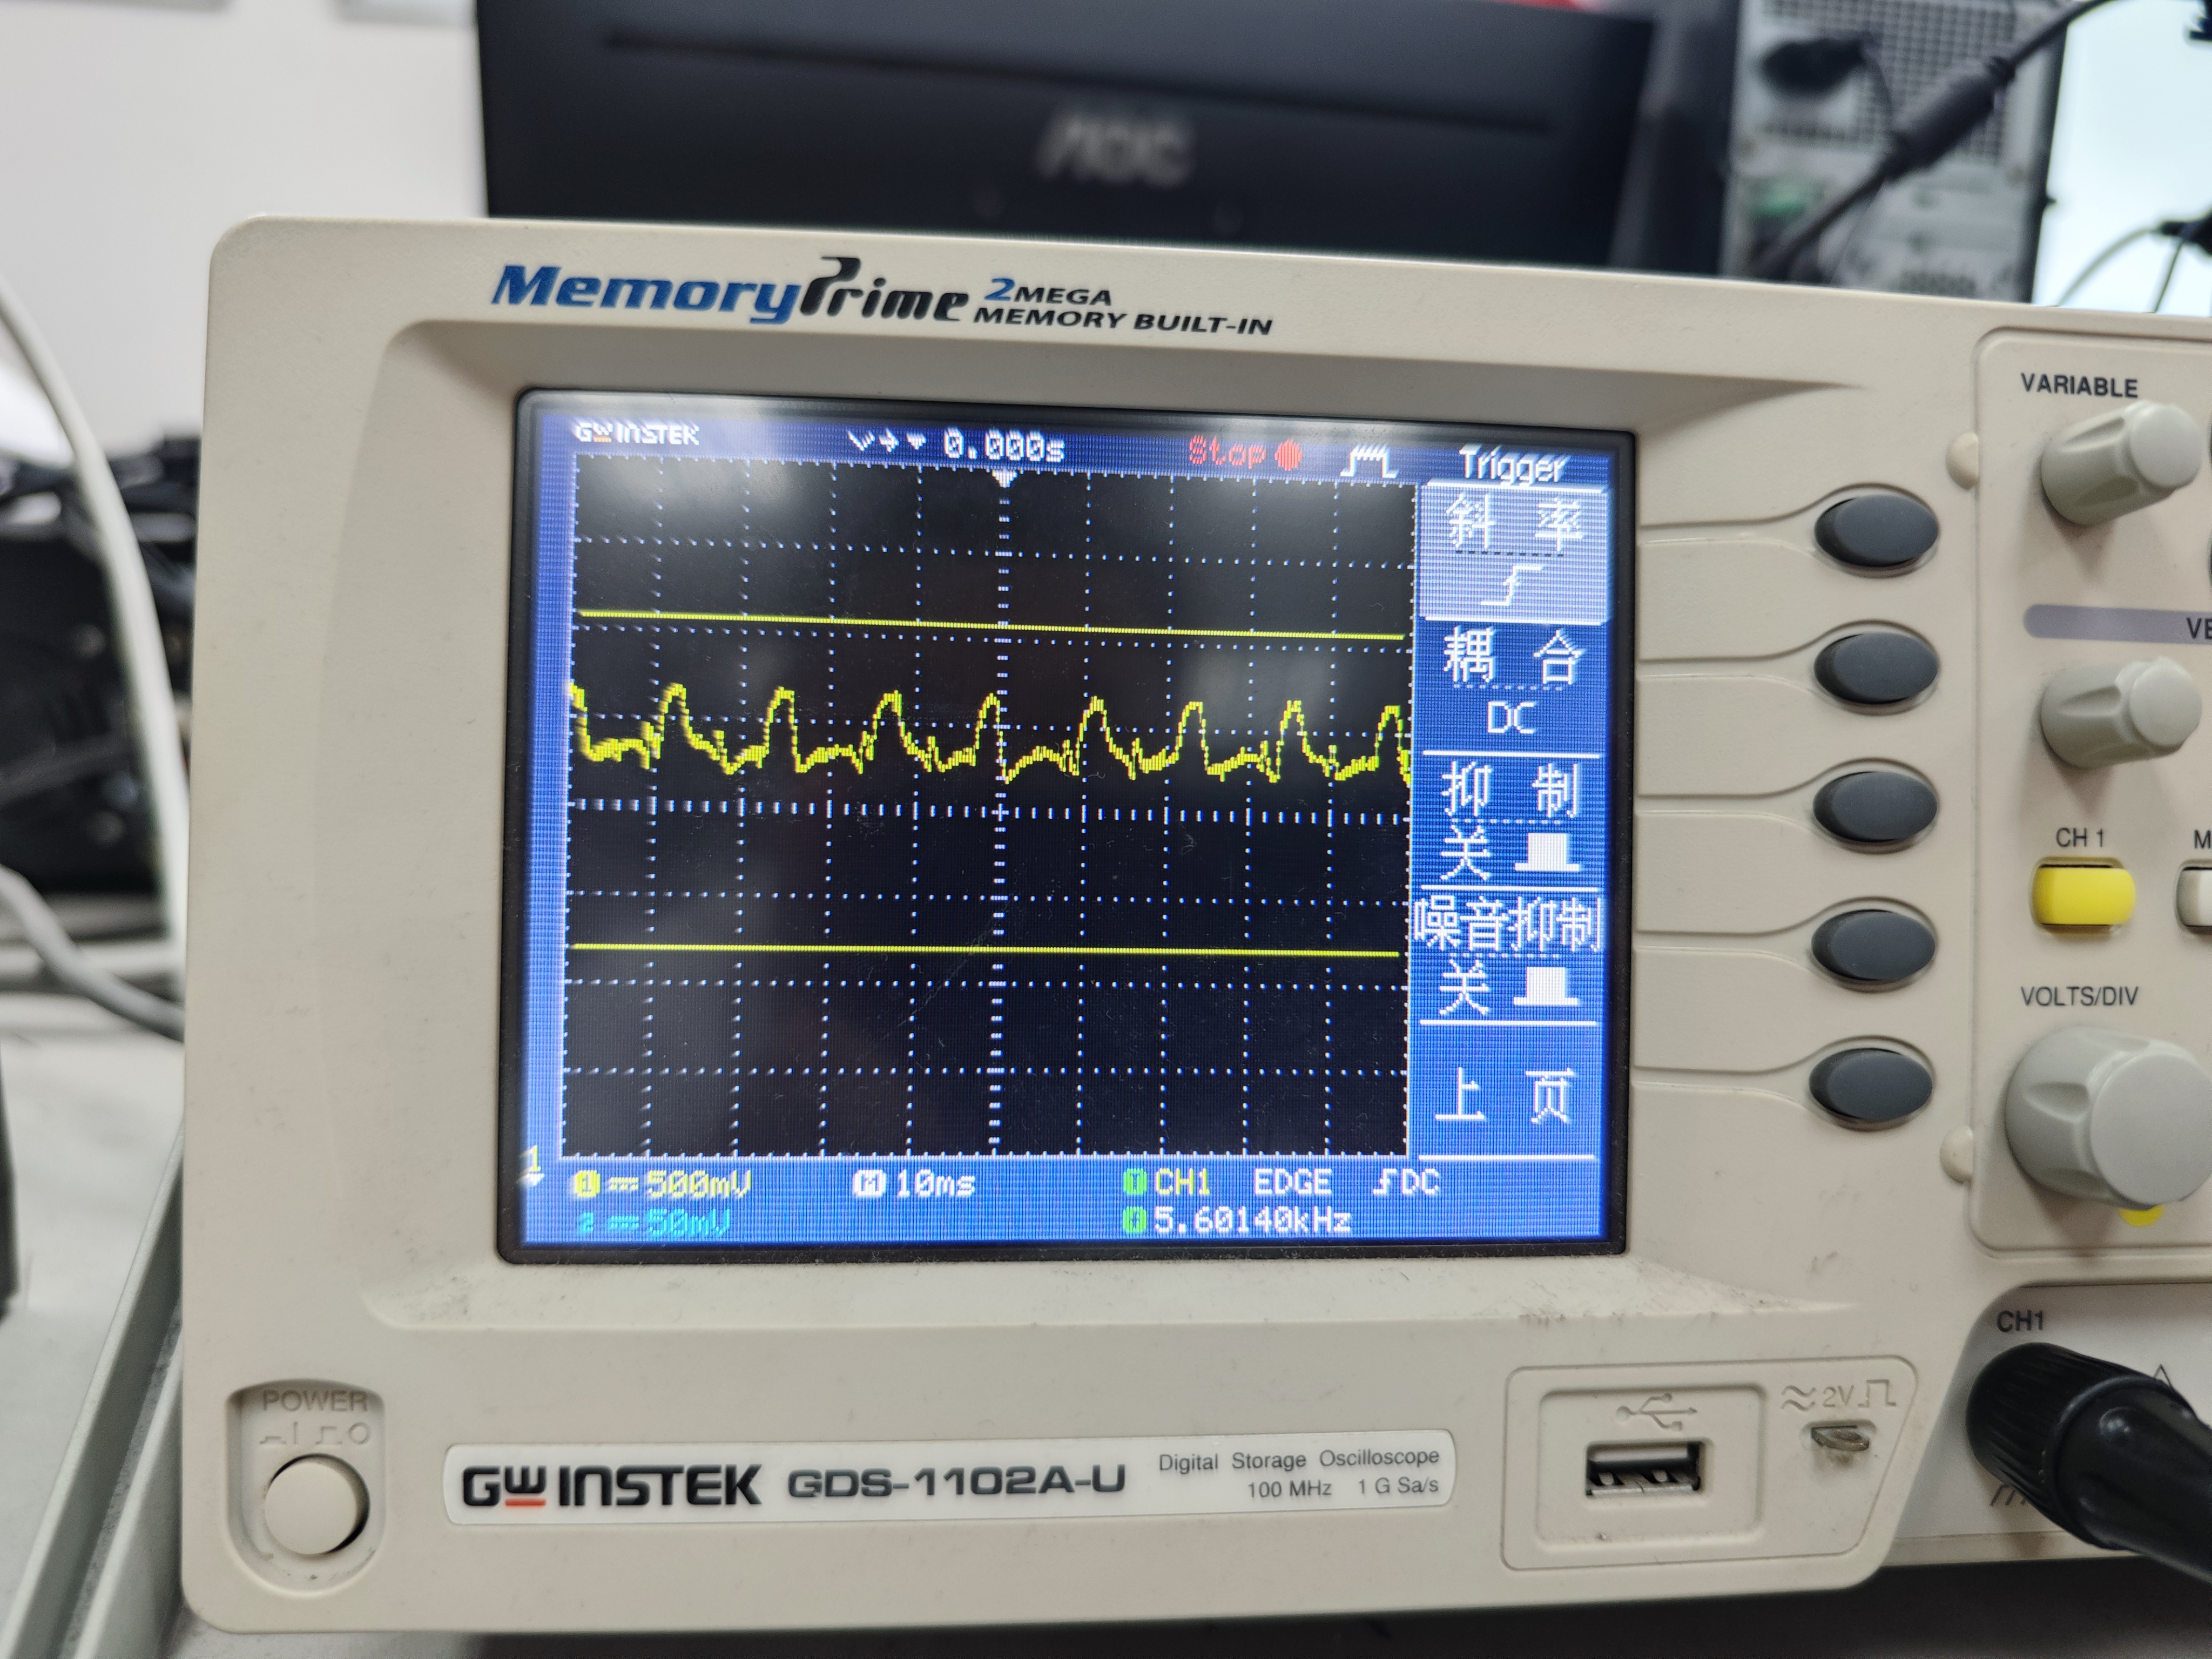
\includegraphics[width=.7\textwidth]{./figures/插座/PWM.jpg}
  \caption{风扇电流值呈周期性变化}
\end{figure}
在测量可调光小台灯及风扇电流的时候,发现其电流一直处于波动状态,可能是因为其使用了PWM技术,导致电流处于周期性波动。
\subsection{软硬件联调任务一}
在智能插座给风扇供电时,电流值不停地大小波动变化,这是风扇采用了PWM技术。为了使得测得的风扇电流趋于平稳,我们采用了\textbf{选择移动平均法}进行电流的处理。
通过\verb|float currents[16]|记录近16个电流值并求取平均值,经测试,这样可以使电流在同一挡位中平稳,并在挡位切换时快速响应。
\begin{lstlisting}[language=C++, caption={任务一}, captionpos=b]
float currents_1[16];//任务一的代码,通过计算最近的16个数值求平均来抹平波动
int head_1 = 0;
float currents_2[16];
int head_2 = 0;
float sum;
//以上是变量声明
Sensor0 = Sensor0 * 0.173793 - 1.02102156;
Sensor1 = Sensor1 * 0.1754680838 - 2.017431873;
currents_1[head_1] = Sensor0;
head_1 = (head_1 + 1) % 16;
sum = 0;
for (int i = 0; i < 16; i++)
{
  sum += currents_1[i];
}
sum /= 16.0;
// send sensor values:
Serial.print("Socket #1 current: ");
Serial.print((float)sum);
Serial.print(" mA");
Serial.print("\t\t");
currents_2[head_2] = Sensor0;
head_2 = (head_2 + 1) % 16;
sum = 0;
for (int i = 0; i < 16; i++)
{
  sum += currents_2[i];
}
sum /= 16.0;
Serial.print("Socket #2 current: ");
Serial.print((float)sum);
Serial.println(" mA");
//以上这段放在loop函数中来实现电流的计算和输出
\end{lstlisting}
\subsection{软硬件联调任务三}
本任务采用板载LED进行调试,当按下SW1,智能插座电压被分压,导致电压下降。
本任务通过改变LED灯的变换来调试输出电压下降的情况。
\begin{lstlisting}[language=C++, caption={任务三}, captionpos=b]
if(Sensor2 < 4800)//任务三的代码,Sensor2采集的电压值即为智能插座的电压值
{
  digitalWrite(pinLED,HIGH); //D4亮
}else
{
  digitalWrite(pinLED,LOW); //D4灭
}
  \end{lstlisting}
``供电电压突然下降''时,小台灯必须处于点亮状态,若小台灯不点亮则该支路没有电流,分压电阻无法分压,电压将不会有变化。
\subsection{关于按钮}
\begin{table}[H]
\centering
\caption{按钮电压与程序读出值}
\begin{tabular}{L{.3\textwidth}L{.4\textwidth}C{.2\textwidth}}
  \toprule
  检测项目  & 检测结果 & s1按钮的程序读取值(0/1)\\
  \midrule
  电路上电,按下S1按钮并保持,测量S1电平:  & S1脚的电平\underline{3.313}V。这个就是在按下按钮状态下,系统能通过软件检测到的信号。  & 1\\
  电路上电,松开S1按钮,测量S1电平:  & S1脚的电平\underline{0}V。这个就是在松开按钮状态下,系统能通过软件检测到的信号。  & 0\\
  \bottomrule
\end{tabular}
\end{table}
\section{新智能插座DIY系统测试}
\subsection{测试用例一}
\begin{enumerate}[label = \alph*)]
  \item 测试用例描述:

  基本功能
  \item 测试目的:

  测试智能插座连接一个手机的功能
  \item 操作过程及其结果:

  通过手机热点组网进行连接,观察app指示灯的状态以及测试基本功能,发现可以手机可以发送命令
  控制插座的连接状态,也可以测量电压电流值等,基本功能完好,如图(\ref{正常工作})所示。
  通过app读取数据在表(\ref{数据})。
  \begin{table}[htbp]
    \centering
    \caption{用程序读取到的数据}
    \label{数据}
    \begin{tabular}{L{.1\textwidth}C{.15\textwidth}C{.15\textwidth}C{.15\textwidth}C{.15\textwidth}}
      \toprule
      项目  & 温度  & 电流值  & 电压值  & 功率  \\
      \midrule
      台灯 & 30.8\textcelsius & 0.17A & 4.87V & 0.87W \\
      风扇一档 & 30.9\textcelsius & 0.21A & 4.58V & 1.11W \\
      风扇二档 & 30.9\textcelsius & 0.32A & 4.72V & 1.49W \\
      \bottomrule
    \end{tabular}
  \end{table}
  \begin{figure}[htbp]
    \centering
    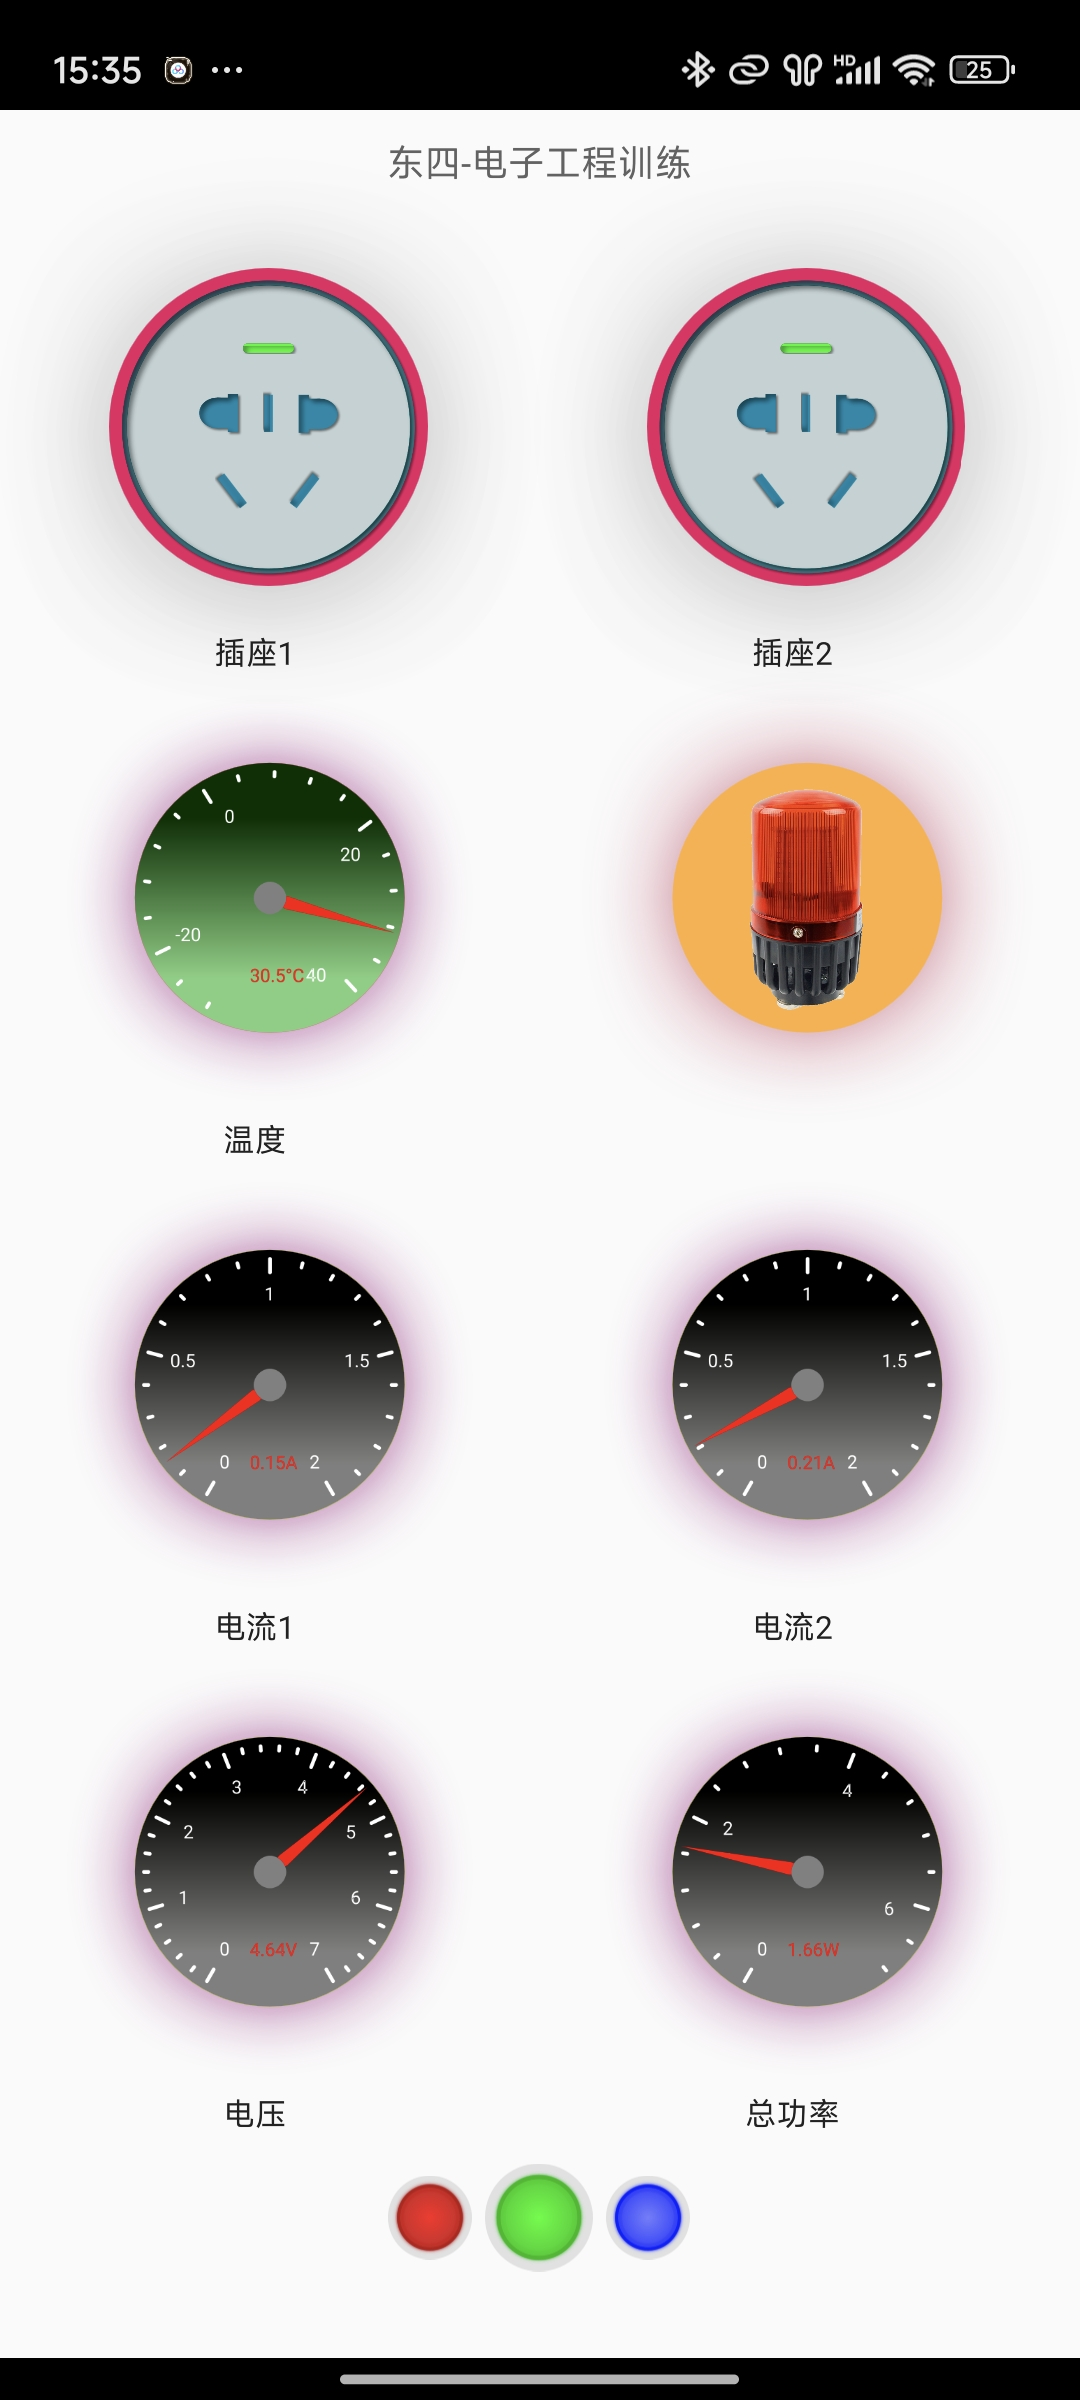
\includegraphics[width=.3\textwidth]{./figures/插座/系统调试/连接.jpg}
    \caption{正常工作}
    \label{正常工作}
  \end{figure}
\end{enumerate}
\subsection{测试用例二}
\begin{enumerate}[label = \alph*)]
  \item 测试用例描述:

  定时开关,延时开关
  \item 测试目的:

  智能插座具备定时开/关、延时开/关的功能
  \item 操作过程及其结果:

  通过设置插座定时,延时,观察开关是否在时间到的时候相应,发现功能完好,如图(\ref{定时})所示。
  \begin{figure}[htbp]
    \centering
    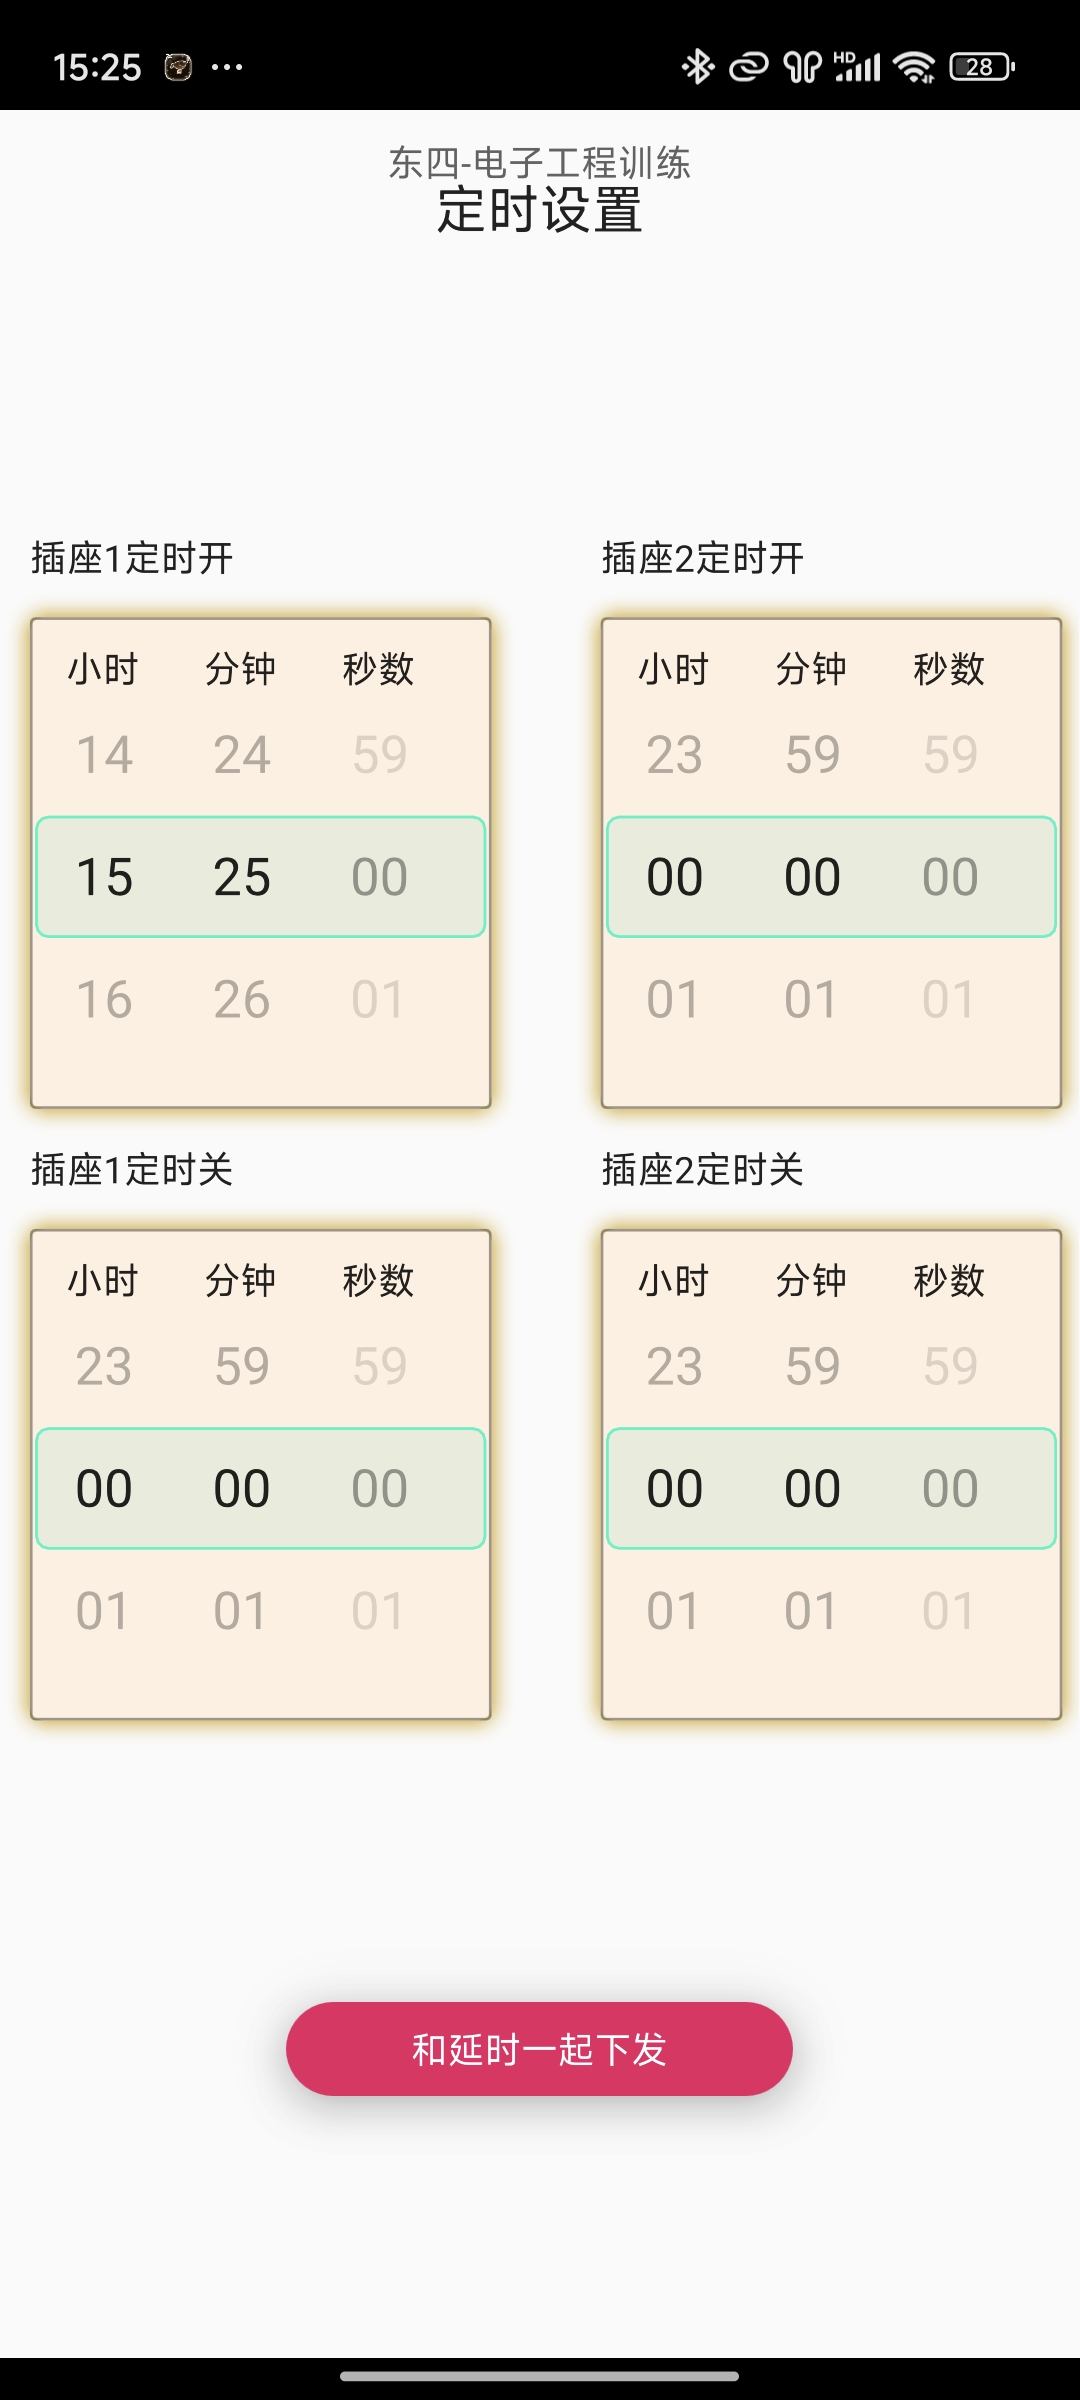
\includegraphics[width=.3\textwidth]{./figures/插座/系统调试/定时.jpg}
    \hspace{5em}
    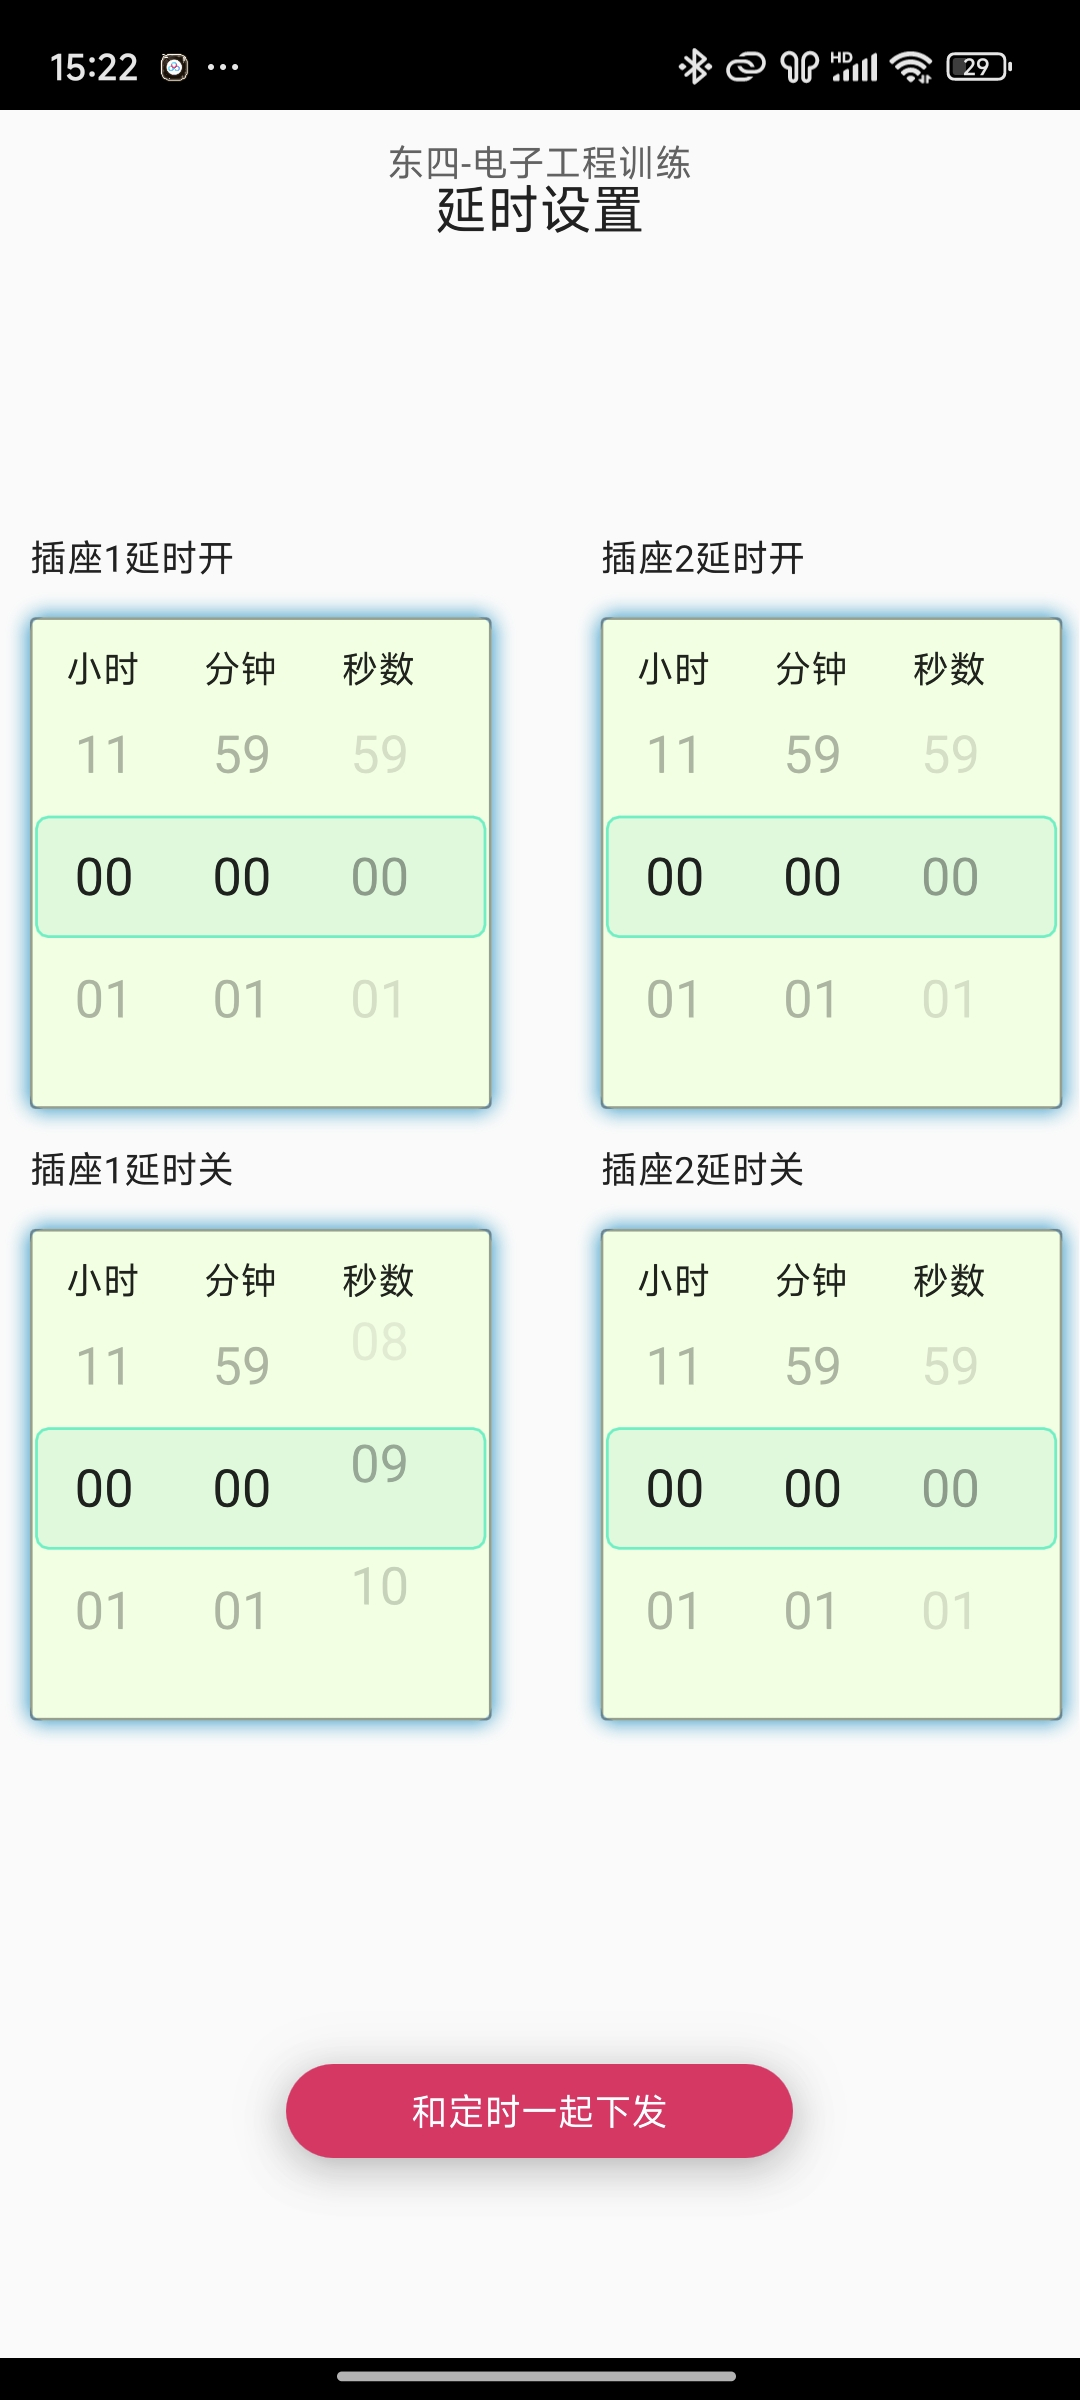
\includegraphics[width=.3\textwidth]{./figures/插座/系统调试/延时.jpg}
    \caption{插座设置定时,延时启动}
    \label{定时}
  \end{figure}
\end{enumerate}
\subsection{测试用例三}
\begin{enumerate}[label = \alph*)]
  \item 测试用例描述:

  针对超/欠电压、超电流、超功率告警并自动断开插座供电。
  \item 测试目的:

  测试插座的告警功能。
  \item 操作过程及其结果:
  \begin{enumerate}
    \item 测试子项目:超/欠电压

    测试过程:先保持下限设为最低,电压上限设为4.6V,打开插座后立即告警,恢复后将电压下限设为4.2V,上限最高
    并按下SW1使电压下降,发现插座立刻告警并断开供电。如图(\ref{电压})所示。

    \begin{figure}[htbp]
        \centering
        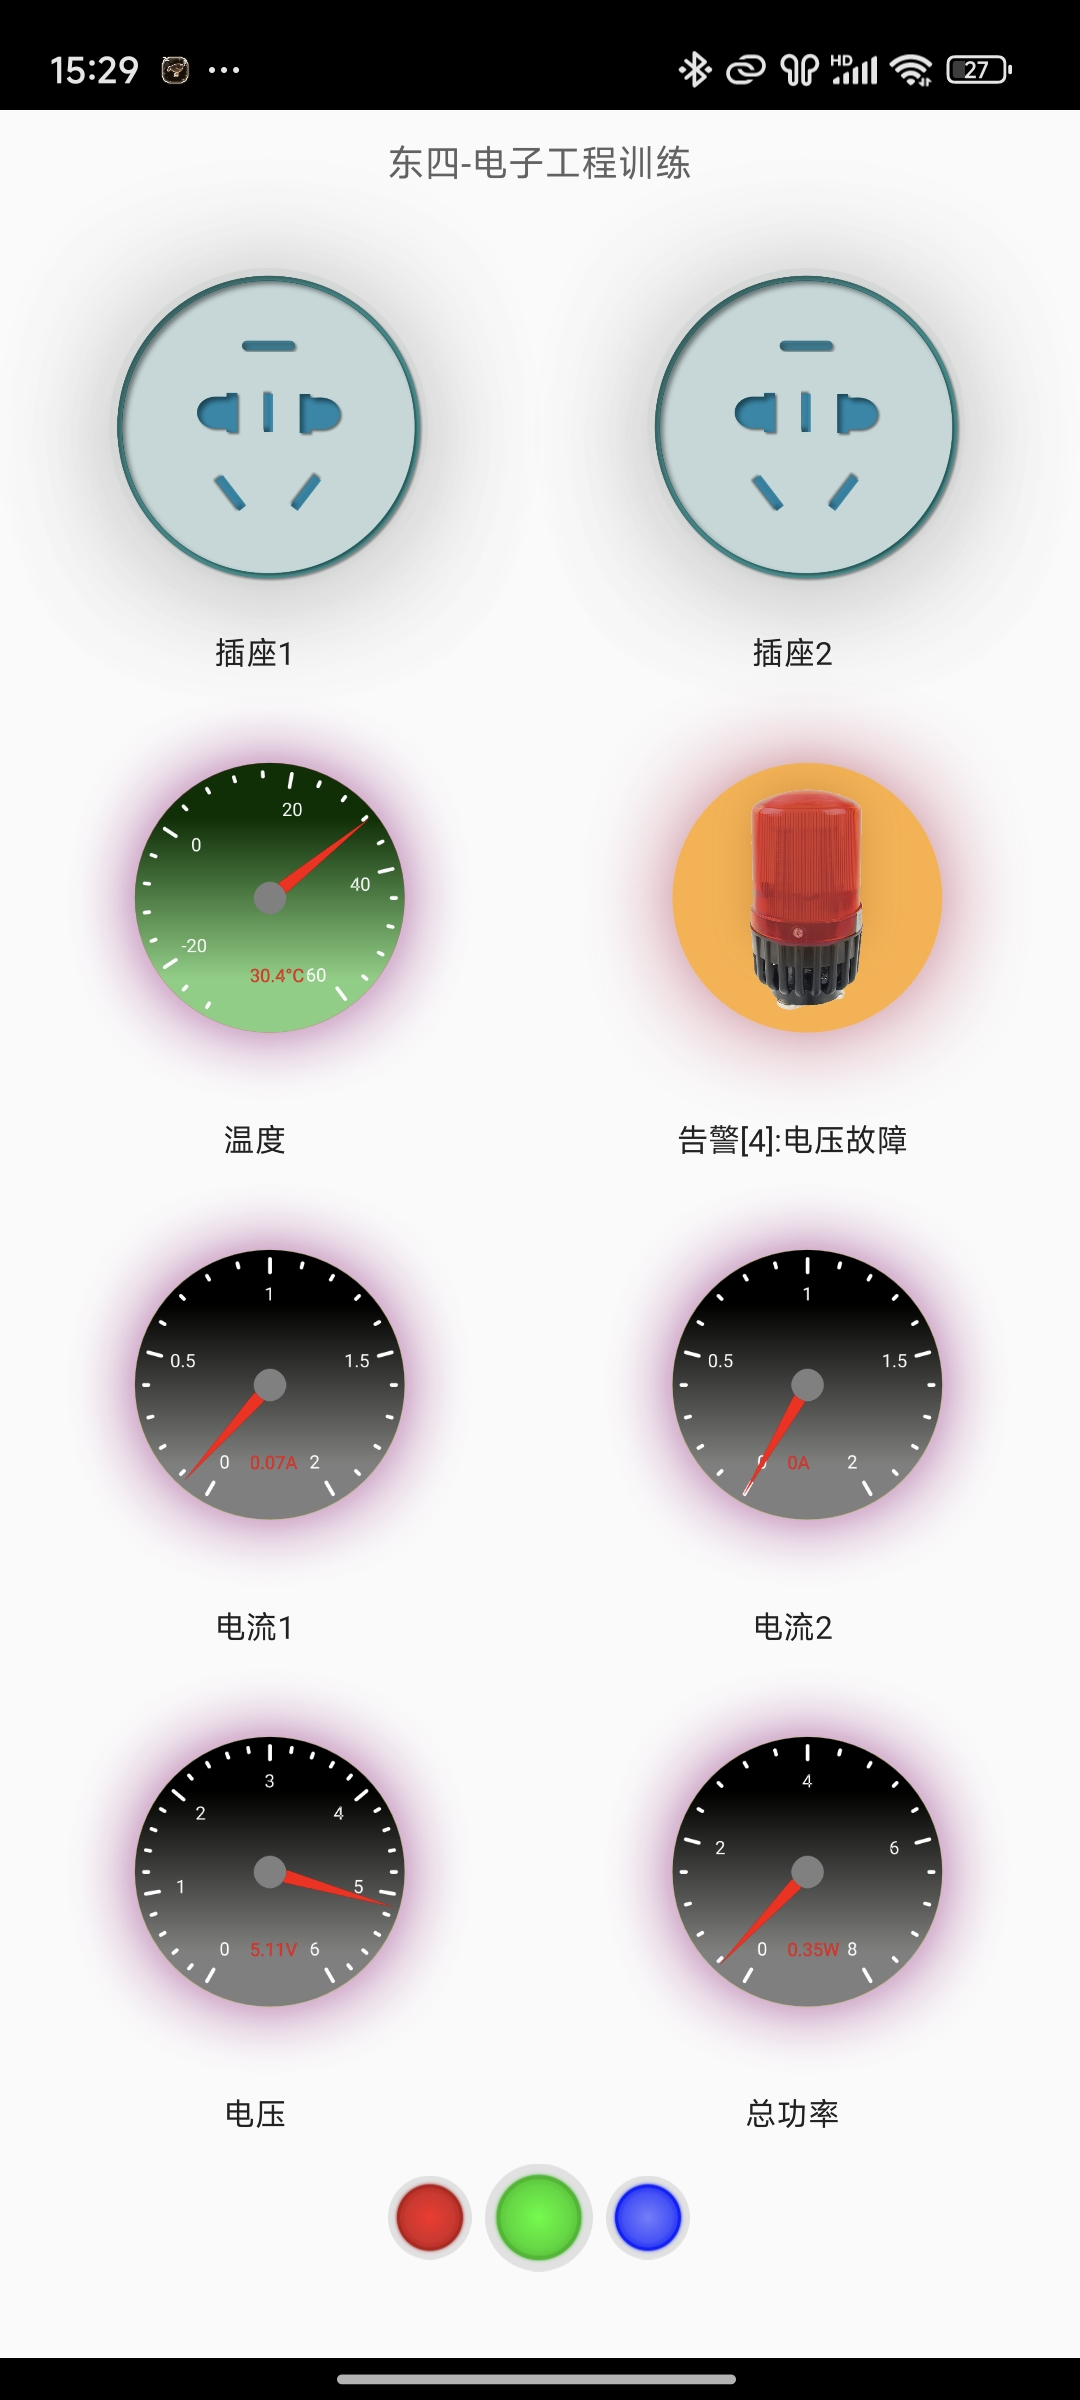
\includegraphics[width=.3\textwidth]{./figures/插座/系统调试/电压超限.jpg}
        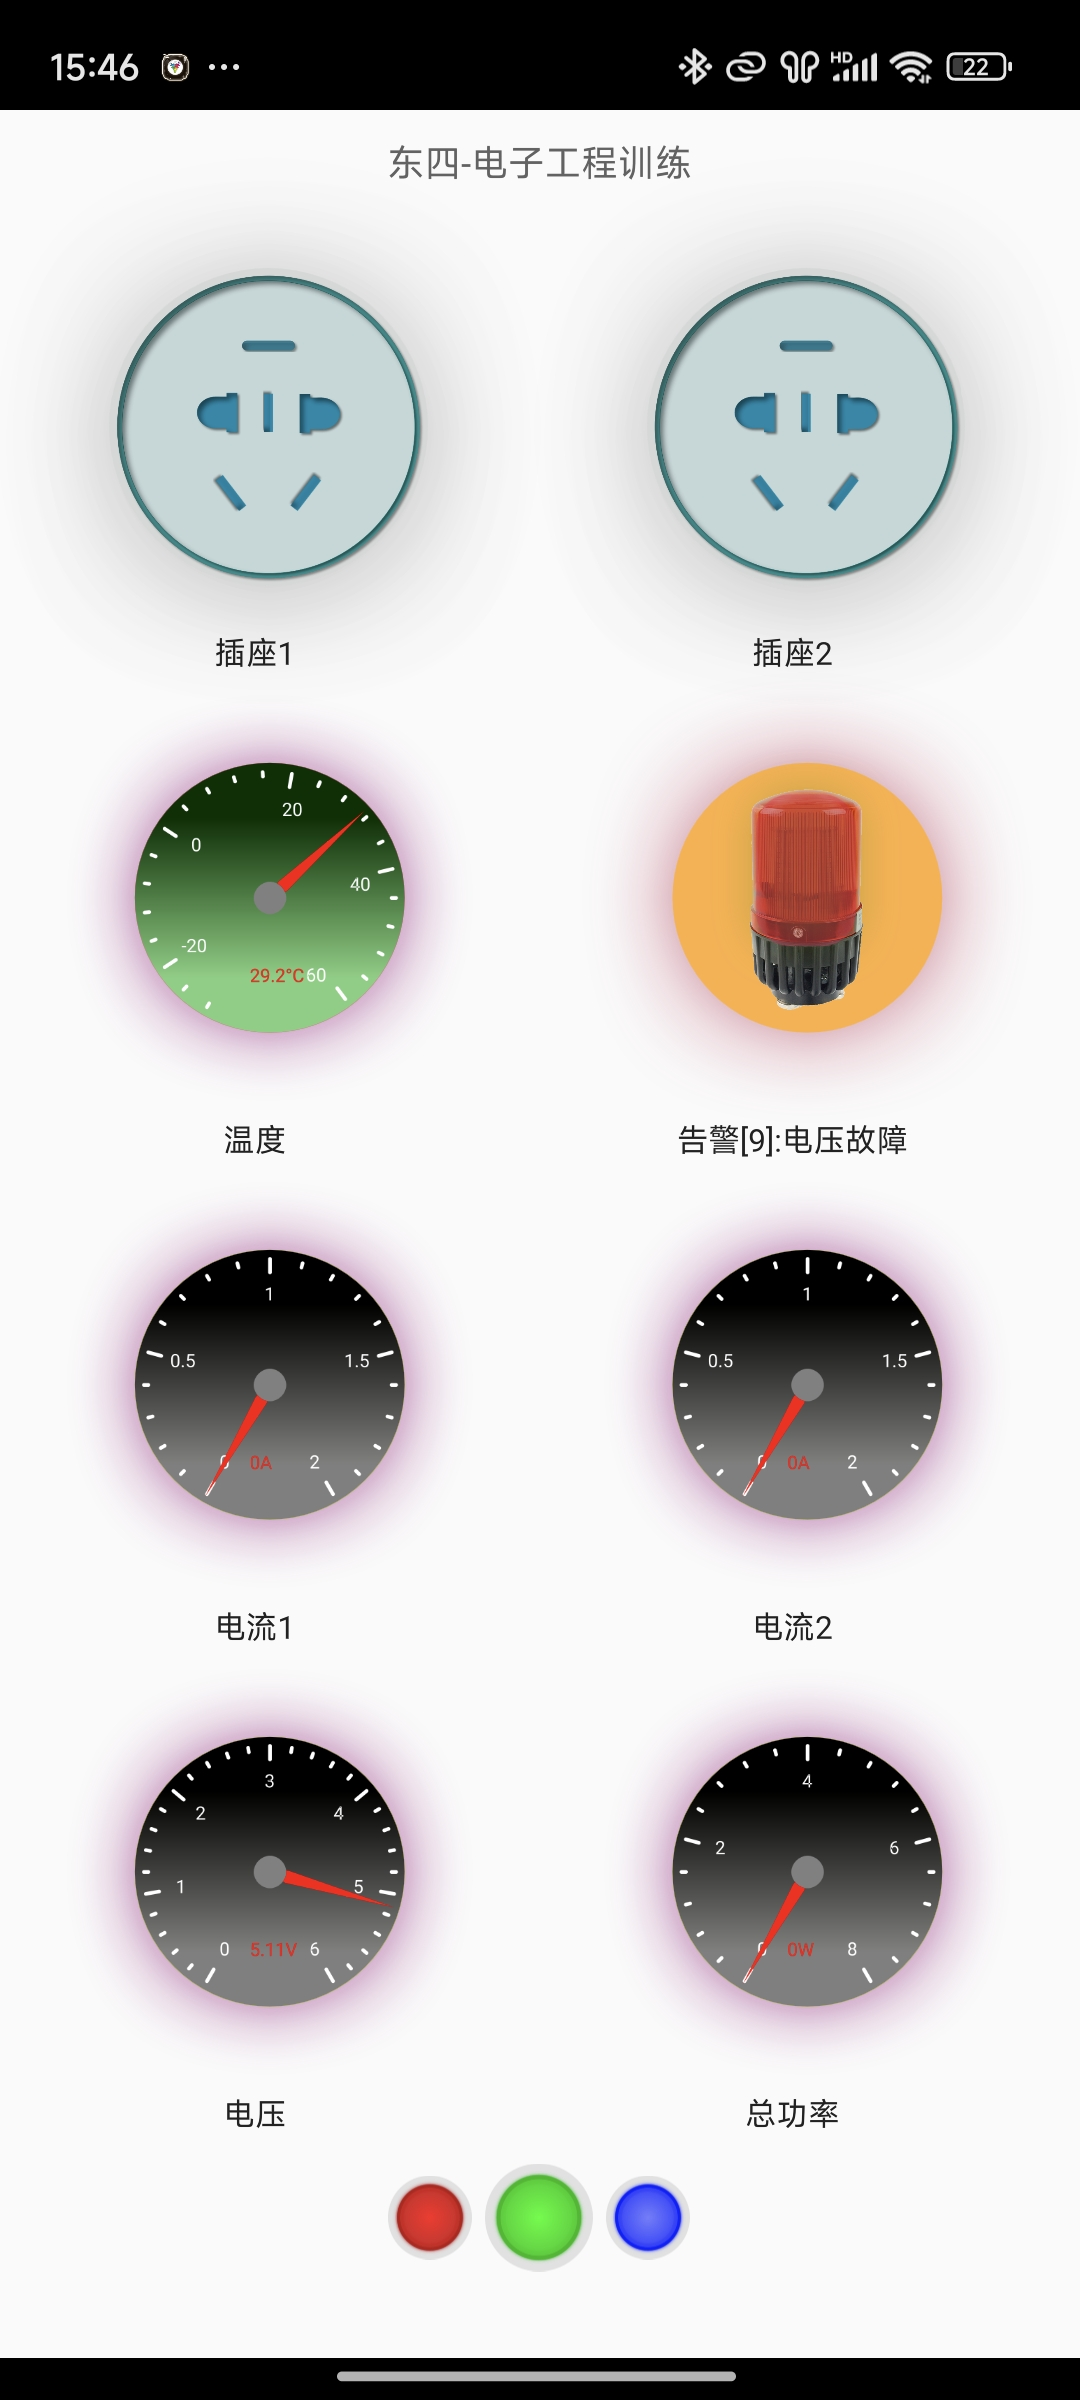
\includegraphics[width=.3\textwidth]{./figures/插座/系统调试/电压过低.jpg}
        \caption{插座关于电压的告警}
        \label{电压}
      \end{figure}

    \item 测试子项目:超电流

    测试过程:设置电流上限为0.1A,接入小风扇并调至三档,立刻给出电流超限告警并断开了插座供电,如图(\ref{电流})所示。

    \begin{figure}[htbp]
        \centering
        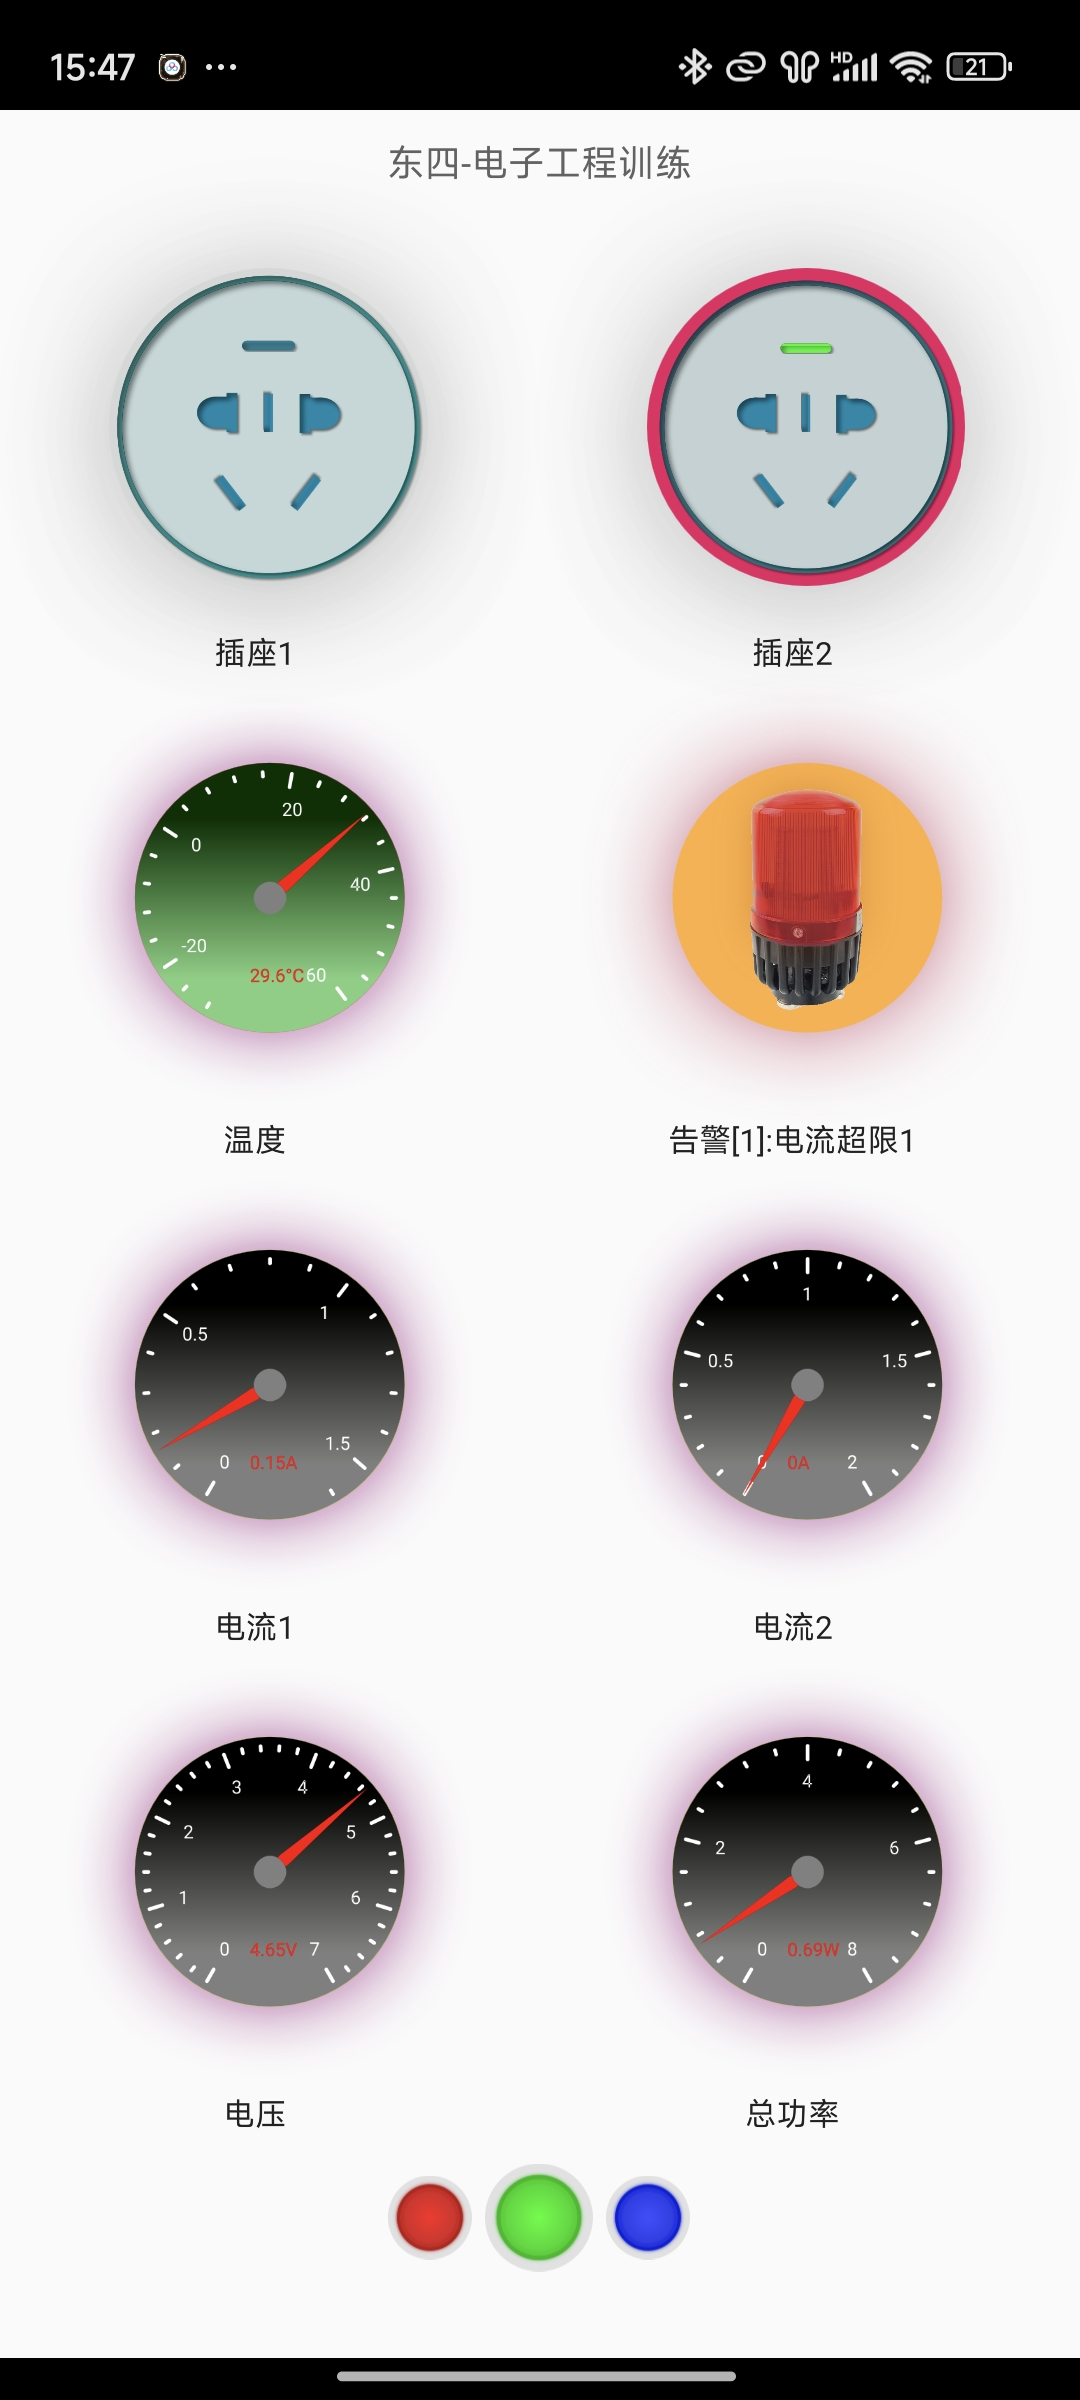
\includegraphics[width=.3\textwidth]{./figures/插座/系统调试/电流超限.jpg}
        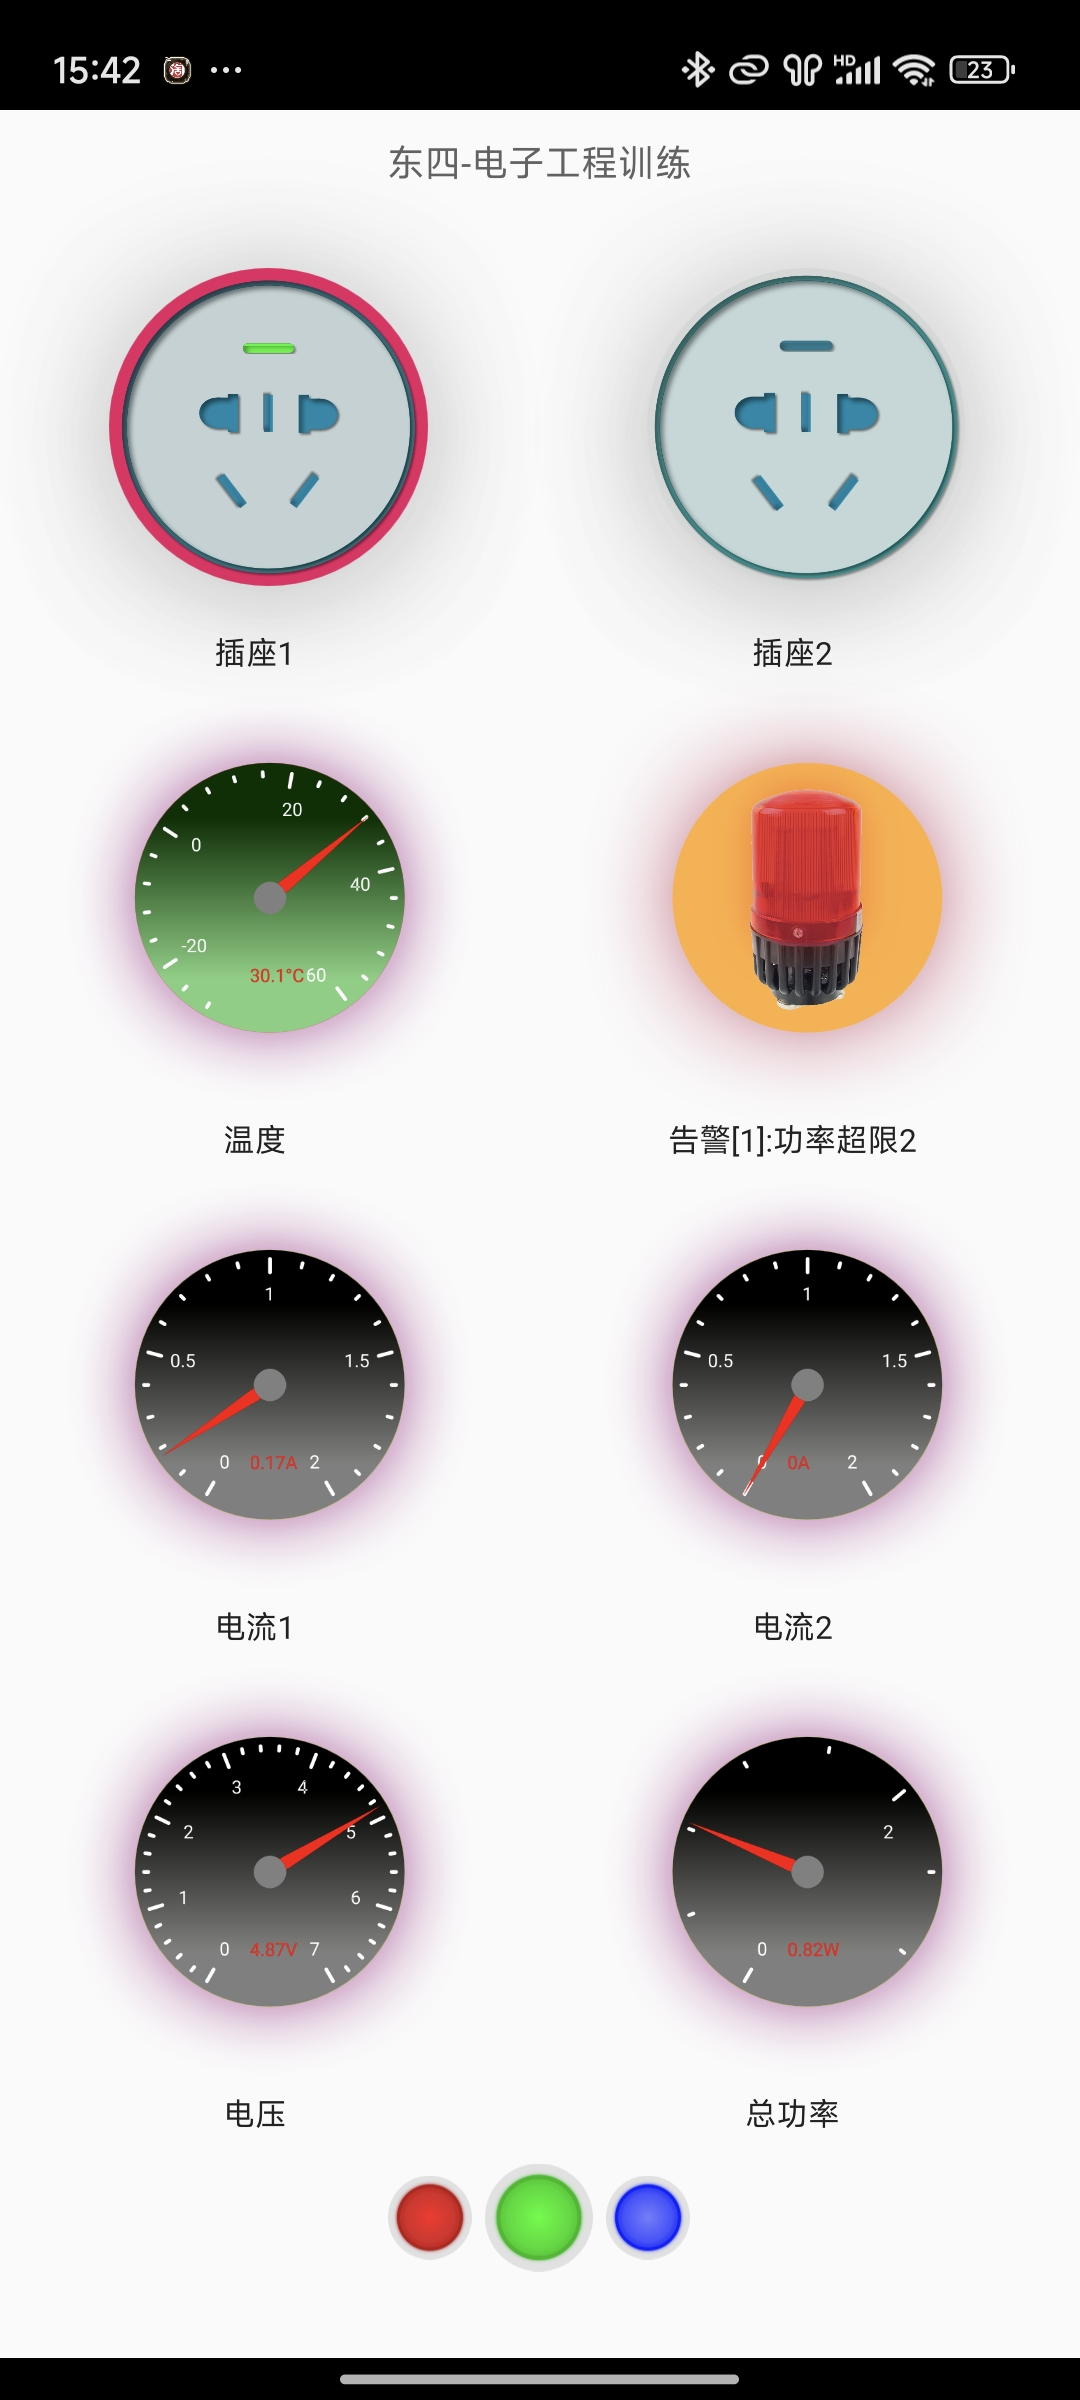
\includegraphics[width=.3\textwidth]{./figures/插座/系统调试/功率超限.jpg}
        \caption{插座关于电流和功率的告警}
        \label{电流}
      \end{figure}

    \item 测试子项目:超功率

    测试过程:设置功率上限为0.5W,接入小风扇并调至三档,立刻给出功率超限告警并断开了插座供电,如图(\ref{电流})所示。
    \item 测试子项目:温度告警

    测试过程:设置温度上限为31\textcelsius,下限设为最低,并用手加热温度传感器,当测量温度值超过设定温度上限时,app给出告警。
    待传感器恢复后将温度上限设为最高值,温度下限设为28\textcelsius,用风扇持续为温度传感器降温,待读数低于设定值时,app同样给出告警,并断开了插座供电,如图(\ref{温度})所示。

    \begin{figure}[htbp]
        \centering
        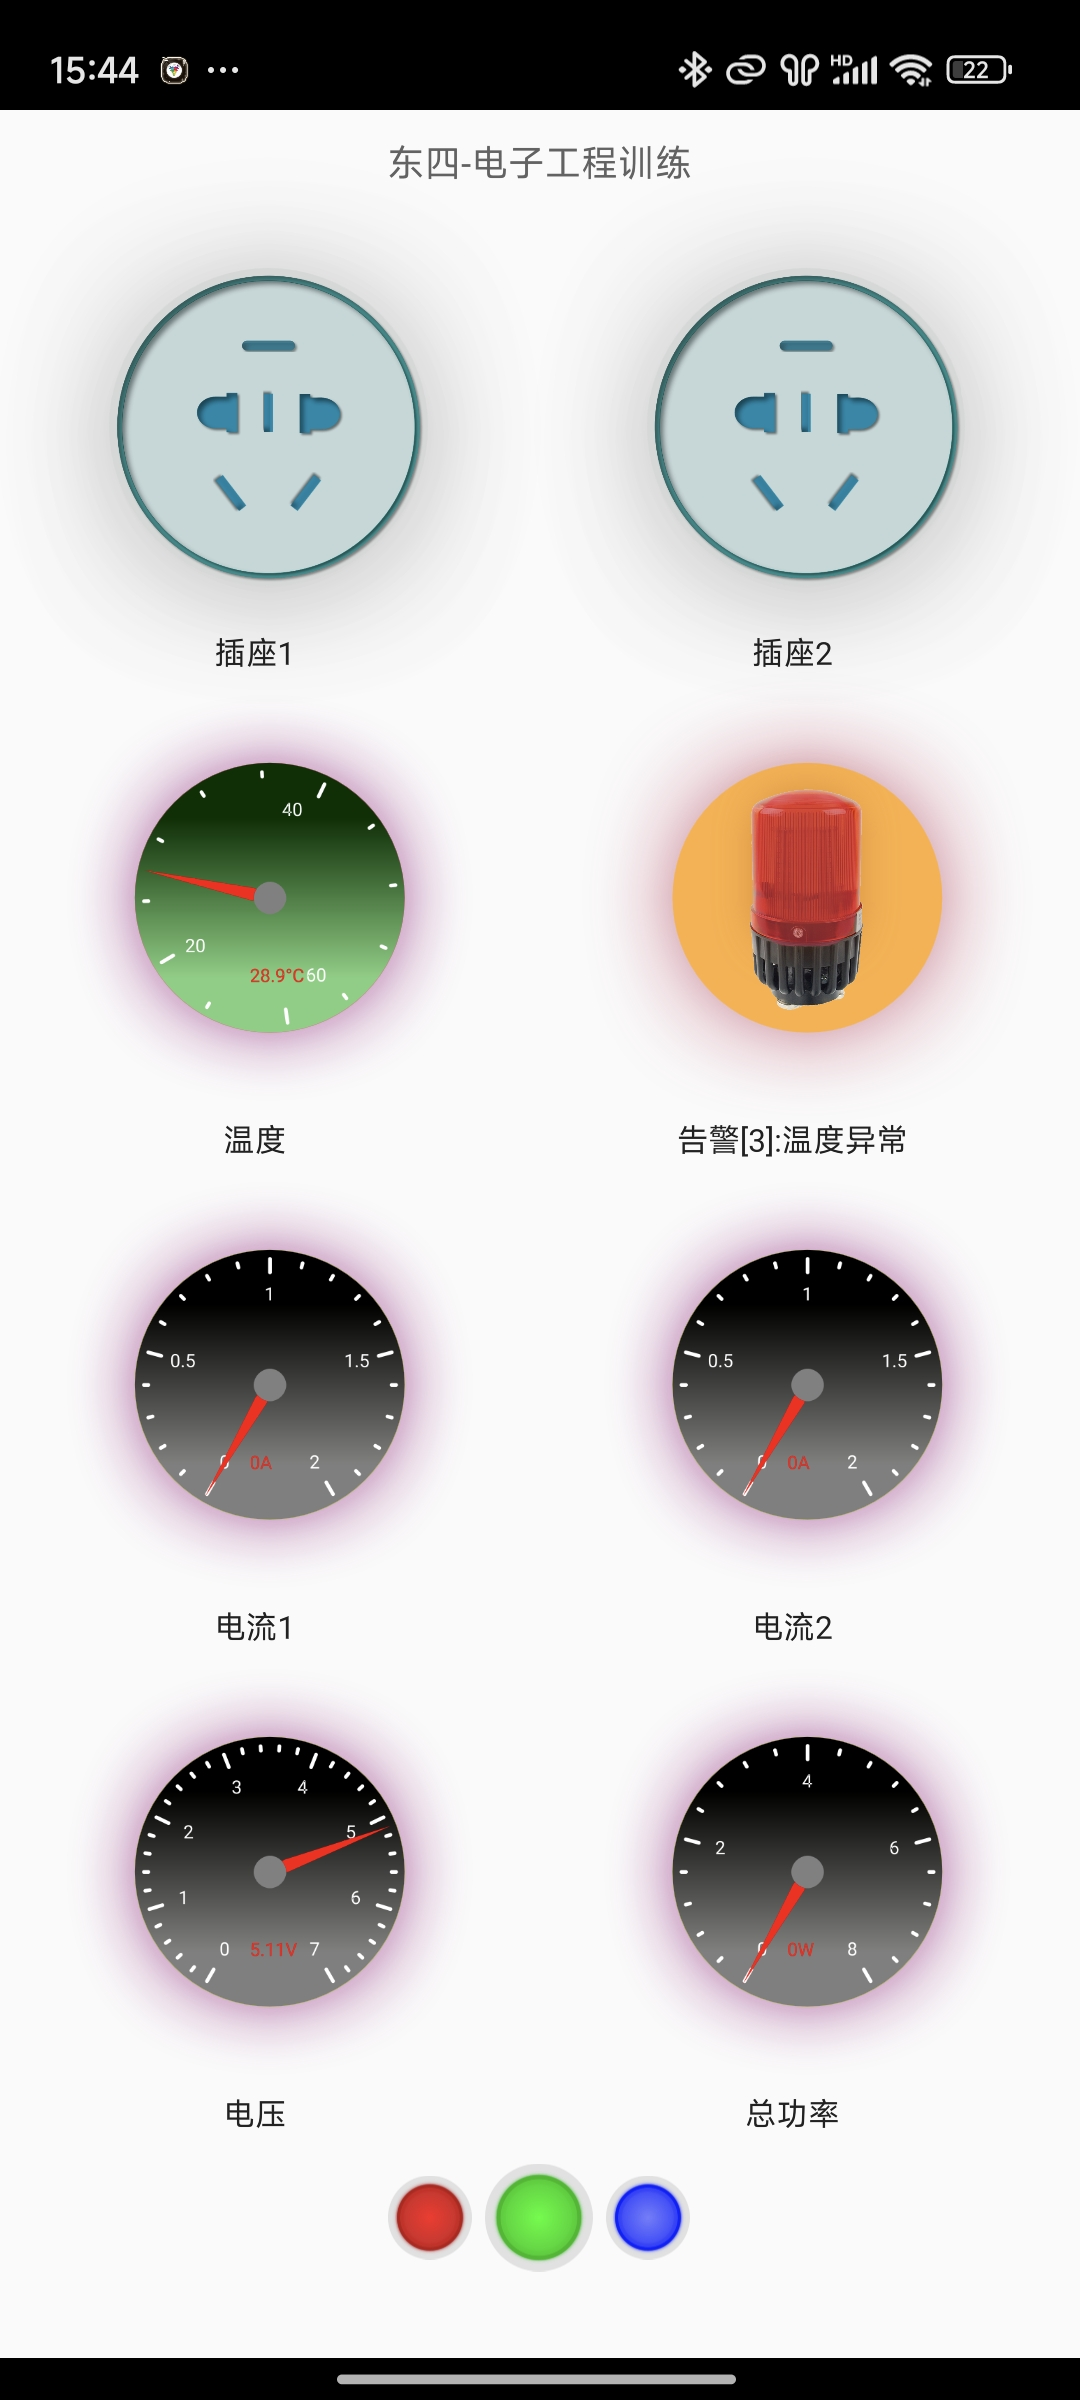
\includegraphics[width=.3\textwidth]{./figures/插座/系统调试/温度过低.jpg}
        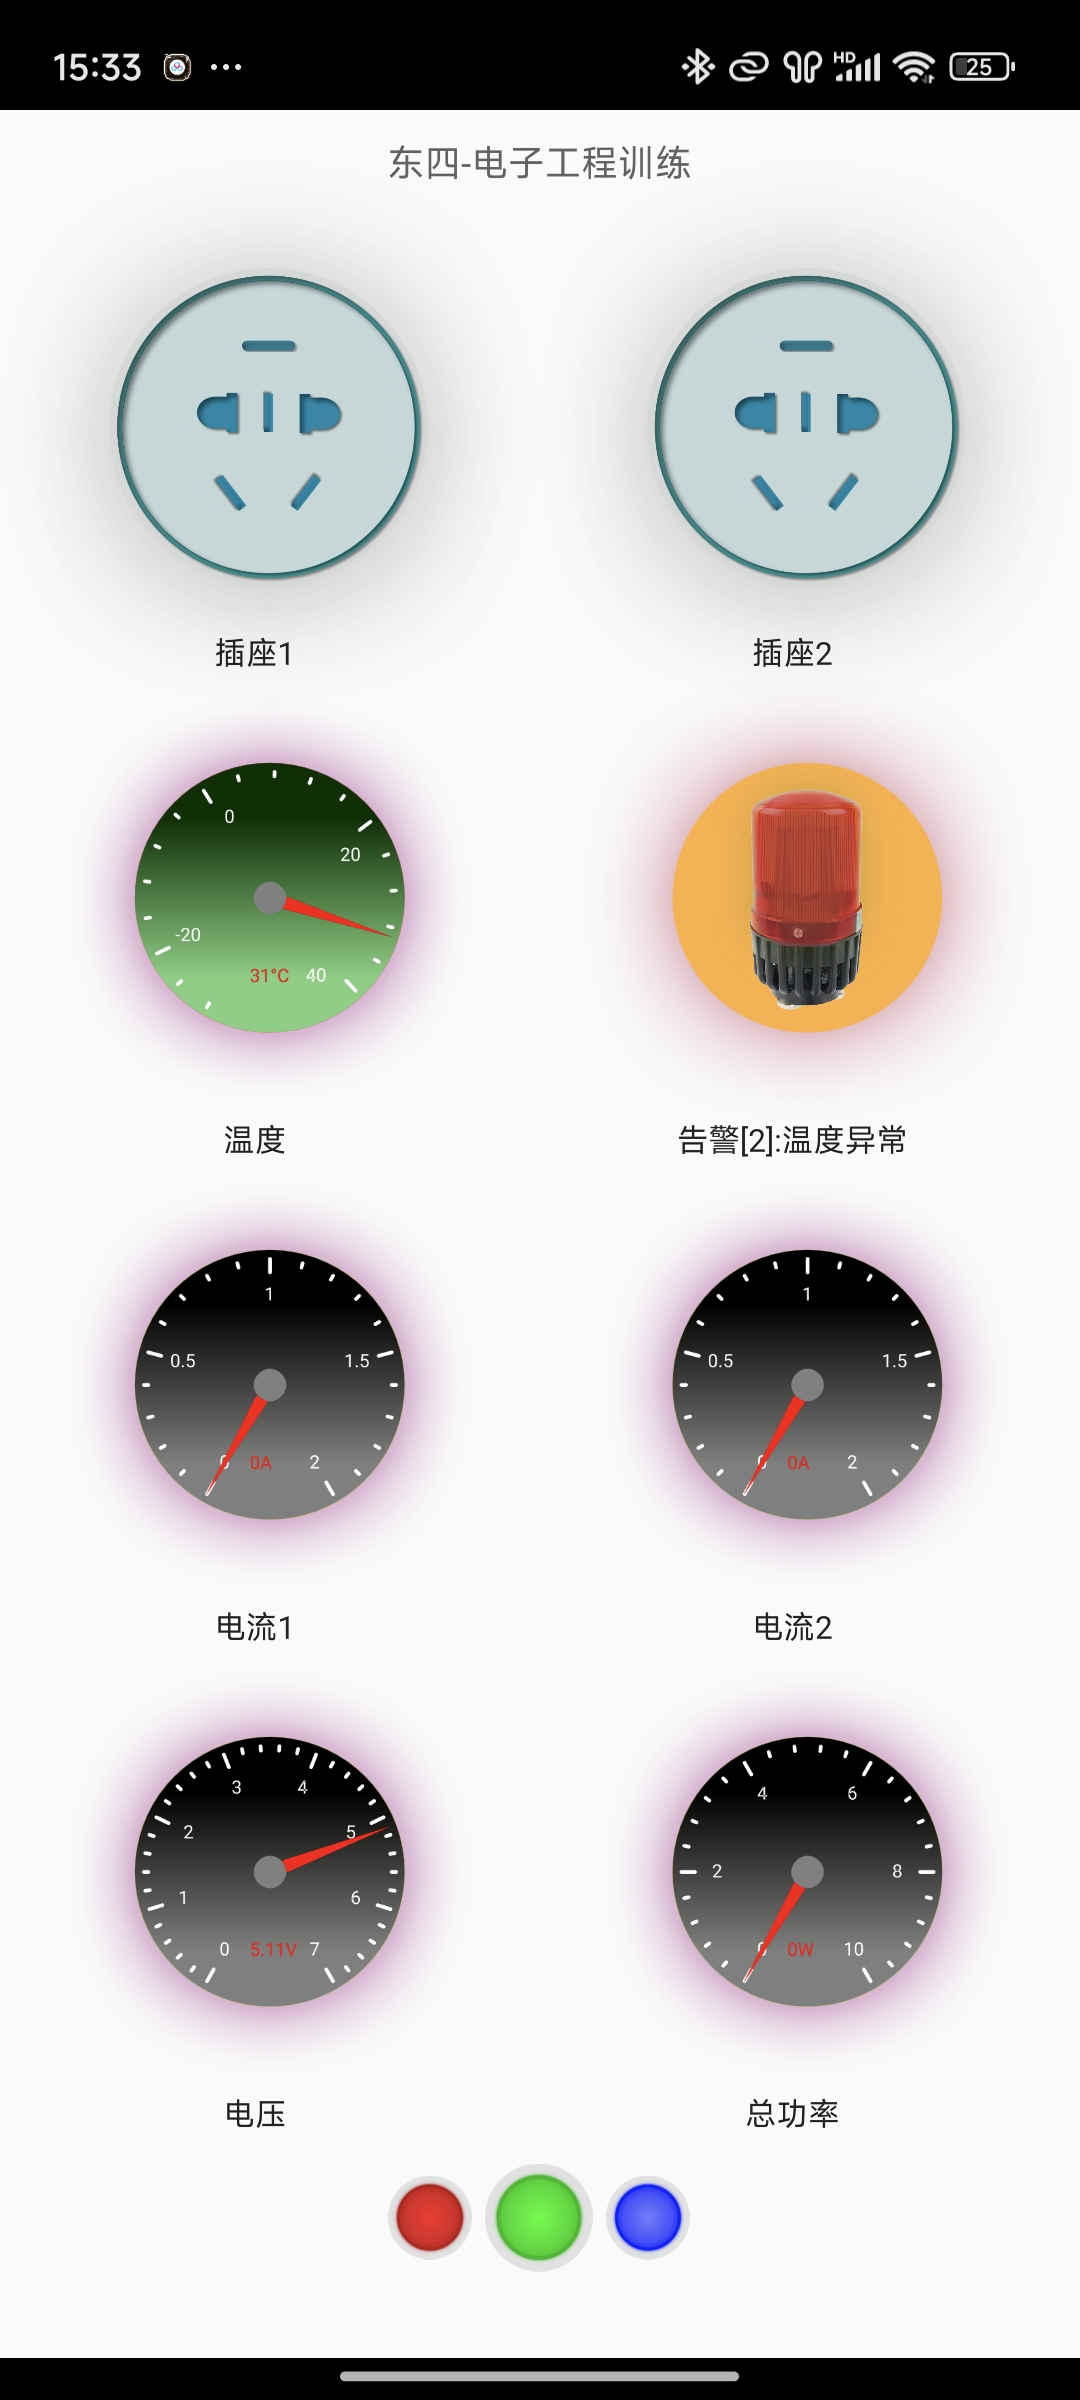
\includegraphics[width=.3\textwidth]{./figures/插座/系统调试/温度过高.jpg}
        \caption{插座关于温度的告警}
        \label{温度}
      \end{figure}
  \end{enumerate}
\end{enumerate}
\end{document}